\chapter{8 TeV Data Selection} \label{ch:data}

Beginning in March of 2012, the LHC began seven months of pp collisions at $\sqrt{s} = \,$ 8 TeV. During the seven months of taking data, the LHC spent 60\% of the time in a state of stable beams as seen in Figure \ref{fig:RunEffer}.

\begin{figure}[h]
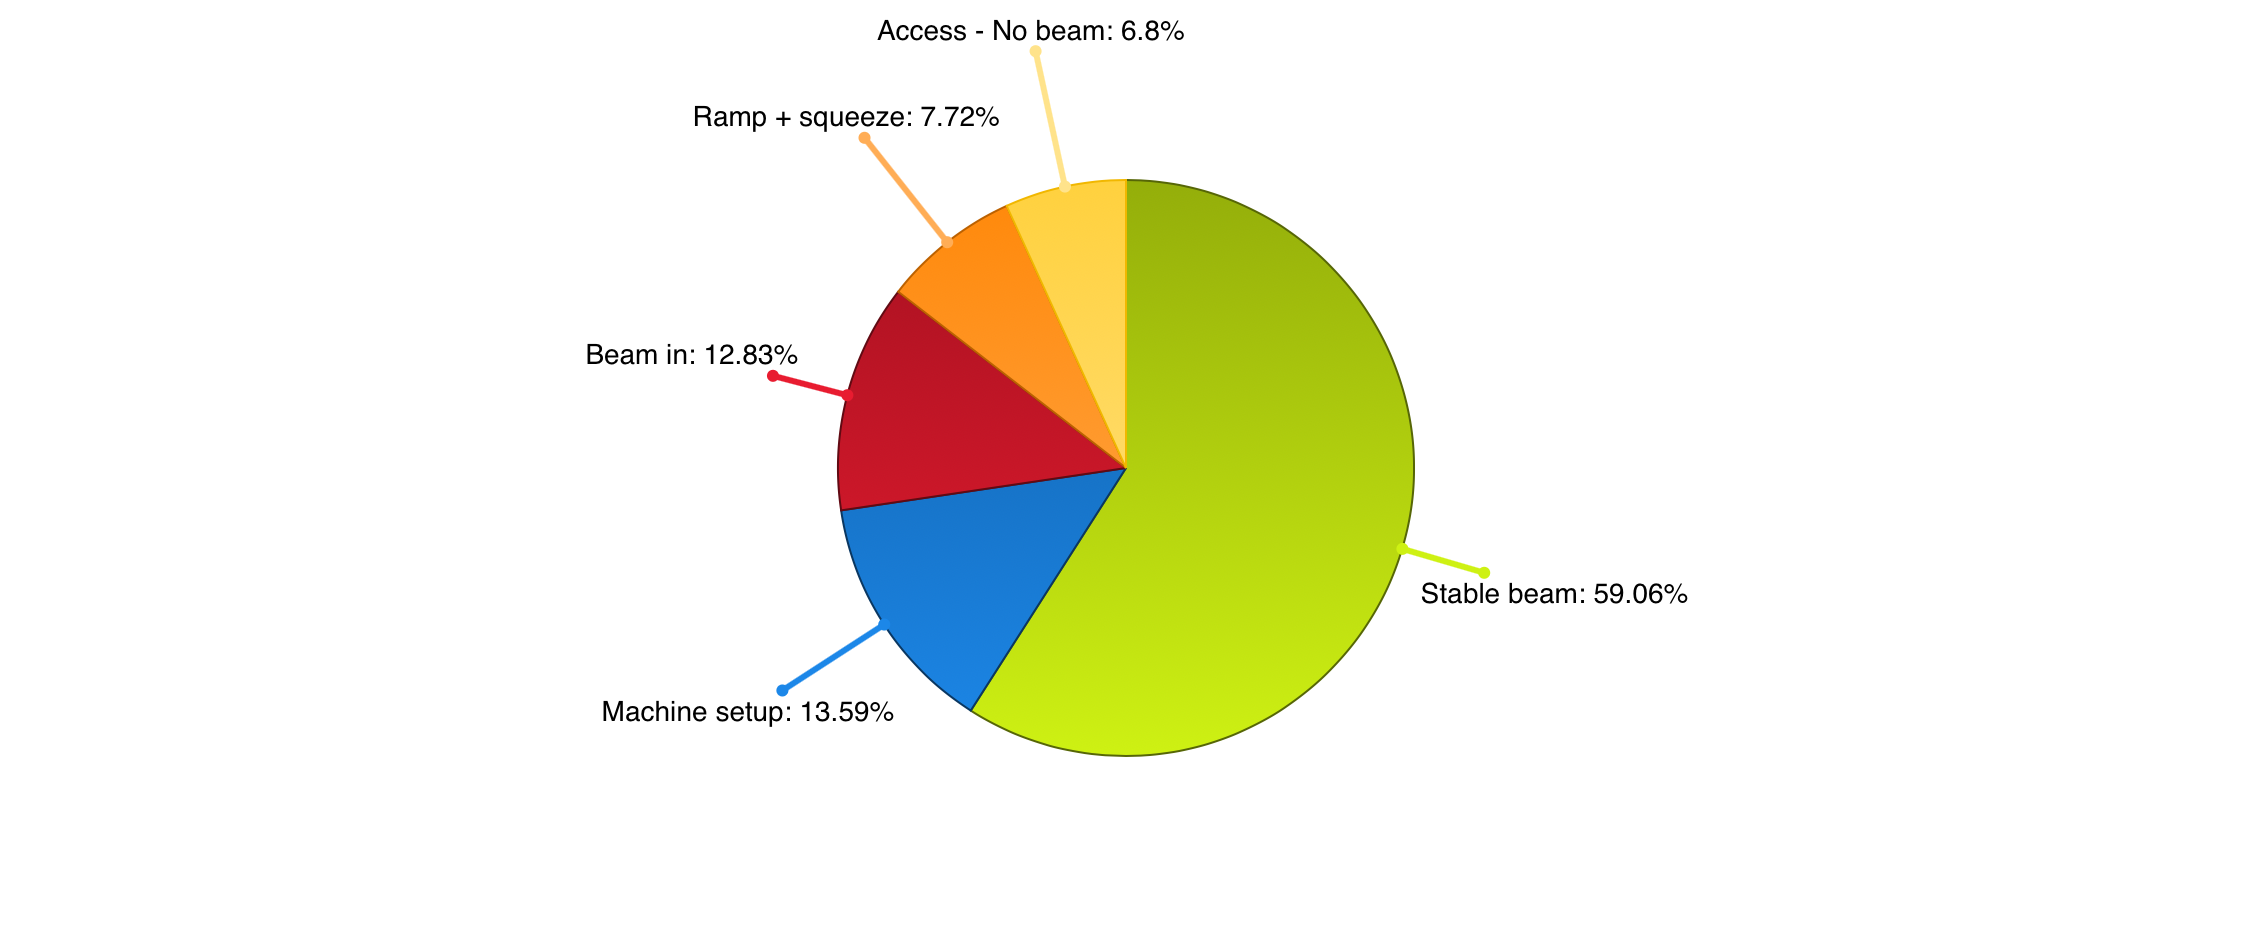
\includegraphics[width=17cm]{8TeVRunefficency}
\centering
\caption{LHC state during the 8 TeV run. }
\label{fig:RunEffer}
\end{figure}


The proton-proton Min Bias trigger is satisfied with at least one hit recorded in the SPD or V0.  ALICE recorded almost 200 million events from this period that satisfied the Min Bias trigger.  ALICE also recorded almost 20 million high-$p_{T}$ events triggered from the EMCal.  Any overview of the EMCal trigger is given in Chapter \ref{ch:alice}.

ALICE is a state-of-the-art experiment with excellent tracking and particle identification capabilities, as discussed in Chapter \ref{ch:alice}.  However, just like any real world experiment, it contains a number of inefficiencies and imperfections.  This means that the data collected during the 8 TeV pp collisions must be examined and any inaccuracies in the data must be removed before any conclusions may be reached.  Data may be compromised at either the event-level, the experiment erroneously recorded something as an event, or at the constituent-level, one of the subdetectors mismeasured a feature of a particle.  The remainder of this chapter focuses on the corrections and quality assurance performed on the 8 TeV data.



\section{Min Bias and EMCal Triggered Events}

During the 8 TeV data collection period, approximately 180 million Min Bias events were recorded, as summarized in table 5.1.  These events were separated into periods, which dictate the particular beam and detector configurations used.  The 8 TeV data was divided into 7 periods, which were further parsed into runs.  A period defines a particular configuration that the ALICE detector or LHC was in.  Periods can differ from another in terms of types of particles colliding, collision energies, trigger conditions, etc. Runs represent an uninterrupted time of data acquisition with ALICE. A run can be as short as 5 minutes or as long as 10 hours.  Runs were separated into `good' runs when both the TPC and EMCal were fully operational, `semi-good runs when a sector of the TPC was turned off but not around the region below the EMCal, and `bad' runs when a portion of the TPC was turned off directly below the EMCal or something else critically compromised the data.  This analysis only incorporated good and semi-good runs.

\begin{table}[hb]
\label{tab:RunSummary}
\begin{center}
\caption{2012 8 TeV data taking period.}
\begin{tabular}[b]{|c|c|c|}
	\hline
	Period & \# of runs & \# of Min Bias events \\ \hline
	LHC12c & 89 & $\sim \,$24 M \\ \hline
	LHC12d & 140 & $\sim \,$62 M \\ \hline
	LHC12e & 5 & $\sim \,$2 M \\ \hline
	LHC12f & 56 & $\sim \,$15 M \\ \hline
	LHC12g & 8 & $\sim \,$0.4 M \\ \hline
	LHC12h & 159 & $\sim \,$75 M \\ \hline
	LHC12i & 40 & $\sim \,$3 M \\ \hline
	Total & 497 & $\sim \,$181 M \\ \hline

\end{tabular}
\end{center}

\end{table}

Approximately 15\% of the data sampled were unusable due to malfunctions in TPC chambers, EMCal super modules, or the electronics of the EMCal or TPC.  The LHC12f and LHC12g EMCal triggered data is not used in this analysis due to a different trigger condition in the EMCal from the other periods.  Besides the bad runs excluded from each of the periods due to QA, the rest of the 8 TeV data was used in this thesis.  The LHC reported the integrated luminosity as $\mathscr{L}_{int} = 8.95 \, pb^{-1}$ for the 8 TeV data\cite{ALICE-PUBLIC-2017-002}.

\subsubsection{Monte Carlo Anchored Data}
Two Monte Carlo data sets which used a full GEANT simulation of the ALICE detector were produced by the ALICE collaboration and used for the Monte Carlo corrections in this analysis.   The first used a Pythia particle-level simulation embedded,in the ALICE GEANT simulation with about 17 million Min Bias generated events. The other uses a PHOjet embed evvents consisting of about 21 million Min Bias triggered events.  Both models used a Min Bias tuning and neither incorporated simulations of the EMCal trigger for high-$p_{T}$ events.

\subsubsection{Event Selection Criteria}
Due to inefficiencies in ALICE it will inevitable contain `bad' events within a data set.  We therefore set a quality assurance criteria by which an event is used in this analysis.  For example, the LHC must be in a state of stable beams, cosmic rays must be excluded by only accepting tracks that originate from a vertex inside the detector, and the relevant detectors for a given analysis must be functioning as intended.  Events were required to meet the following conditions:

\begin{itemize}
  \item The event has a primary vertex reconstructed, this helps exclude cosmic ray events.
  \item The primary vertex occurs within a 10 cm window of the primary interaction point, this maintains our detector acceptance and ensures good particle reconstruction.
  \item The vertex resolution must be below 0.25 cm, this ensures that the vertex is real and not a misreconstruction.
  \item The event passes basic pile-up checks based on the V0 and T0 signals, this ensures that we dont have data from different collisons overlapping one another.
\end{itemize}


A summary of the rejection reasons for an event are shown in Figure \ref{fig:eventqa}.  Most of the rejected events were excluded due to the event not satisfying the vertex requirements.  The vertex rejection does not impose a bias on my final results because these events are low multiplicity and low momentum transfer which have a low probability for jet production.

\begin{figure}[h]
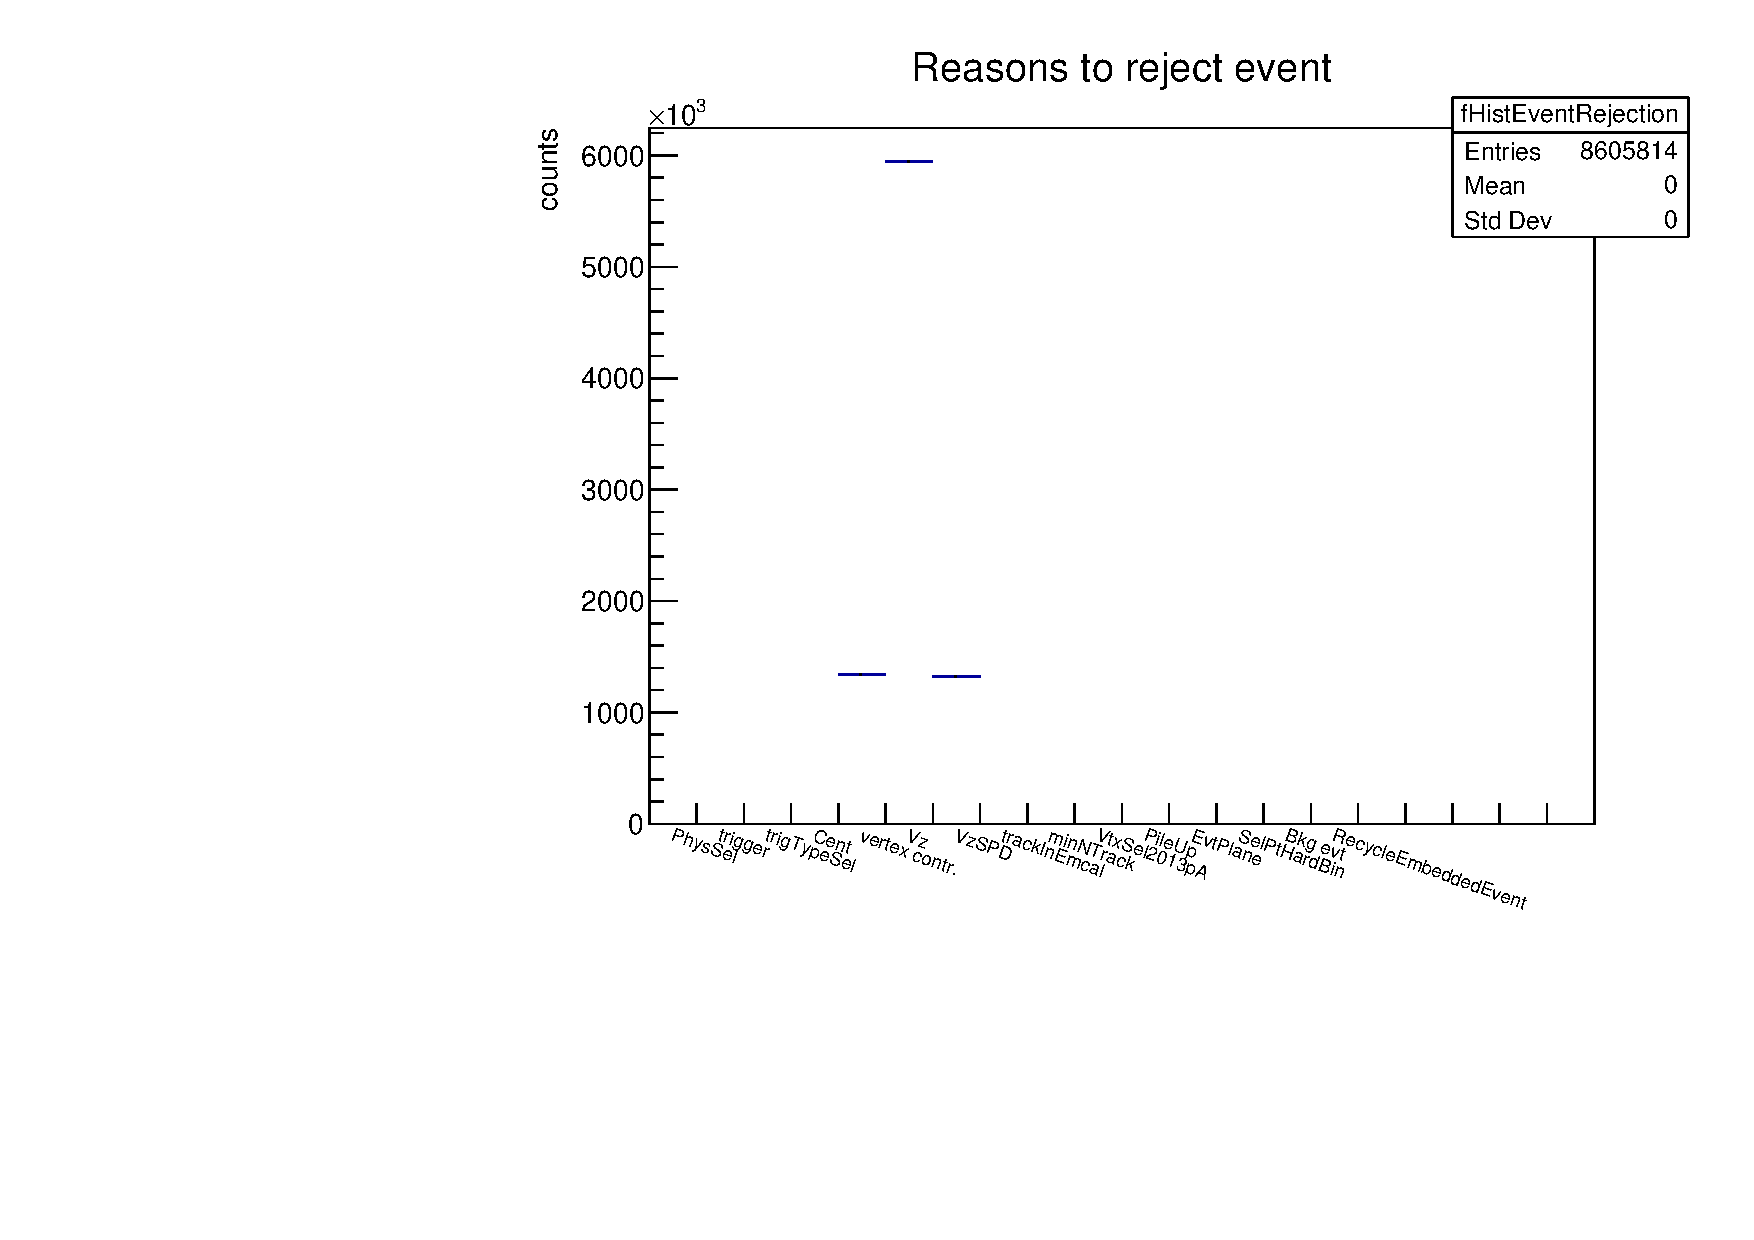
\includegraphics[width=8.5cm]{RejectionReasons}
\centering
\caption{Min Bias event rejection summary.}
\label{fig:eventqa}
\end{figure}

\begin{figure}[h]
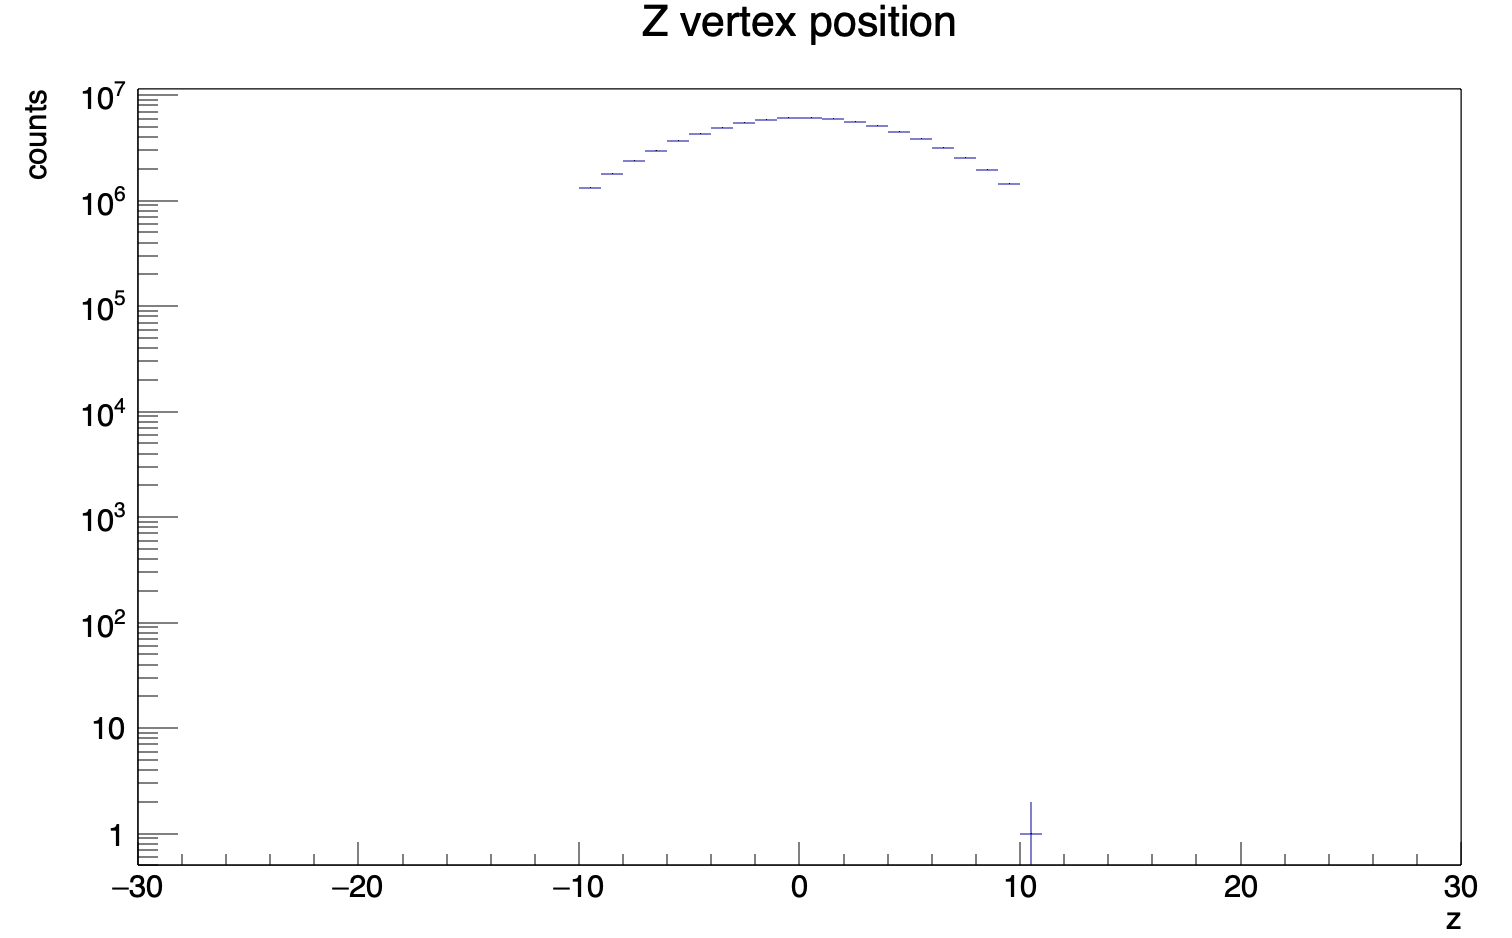
\includegraphics[width=8.5cm]{zvertex}
\centering
\caption{Vertex displacement from primary interaction point for accepted Min Bias events.}
\label{fig:vertrec}
\end{figure}


Figure \ref{fig:vertrec} shows the reconstructed vertex for the accepted Min Bias events.  We see that the vertex distribution peaks at the primary interaction point as expected. 

 In addition to the vertex requirements the 8 TeV data set was investigated for the presence of LED events.  The EMCal uses a system of LEDs for calibrations.  Previous ALICE data sets had events contaminated by the LED firing.  The presence of LED events within the 8 TeV data was investigated by measuring the EMCal cell multiplicity per super-module for each event.  No LED events were found within the 8 TeV data set.
The EMCal triggered data used similar event criteria to the Min Bias data and  triggered most events were rejected due to the vertex requirements.


\section{EMCal Clusters}


Corrections were applied to cells including the removal of hot and dead towers (bad channels) based on the average occupancy and energy of the towers, calibrations to cell timing caused by the physical layout of the EMCal (such as differences in cabling length), and an energy calibration based on the $\pi^{0}$ mass.   Figure \ref{fig:badchannel} shows a bad channel map after removing the hot and dead towers from a typical run.  The $\phi$ distribution is segmented into 5 parts representing the five super modules of the EMCal.  

\begin{figure}[h]
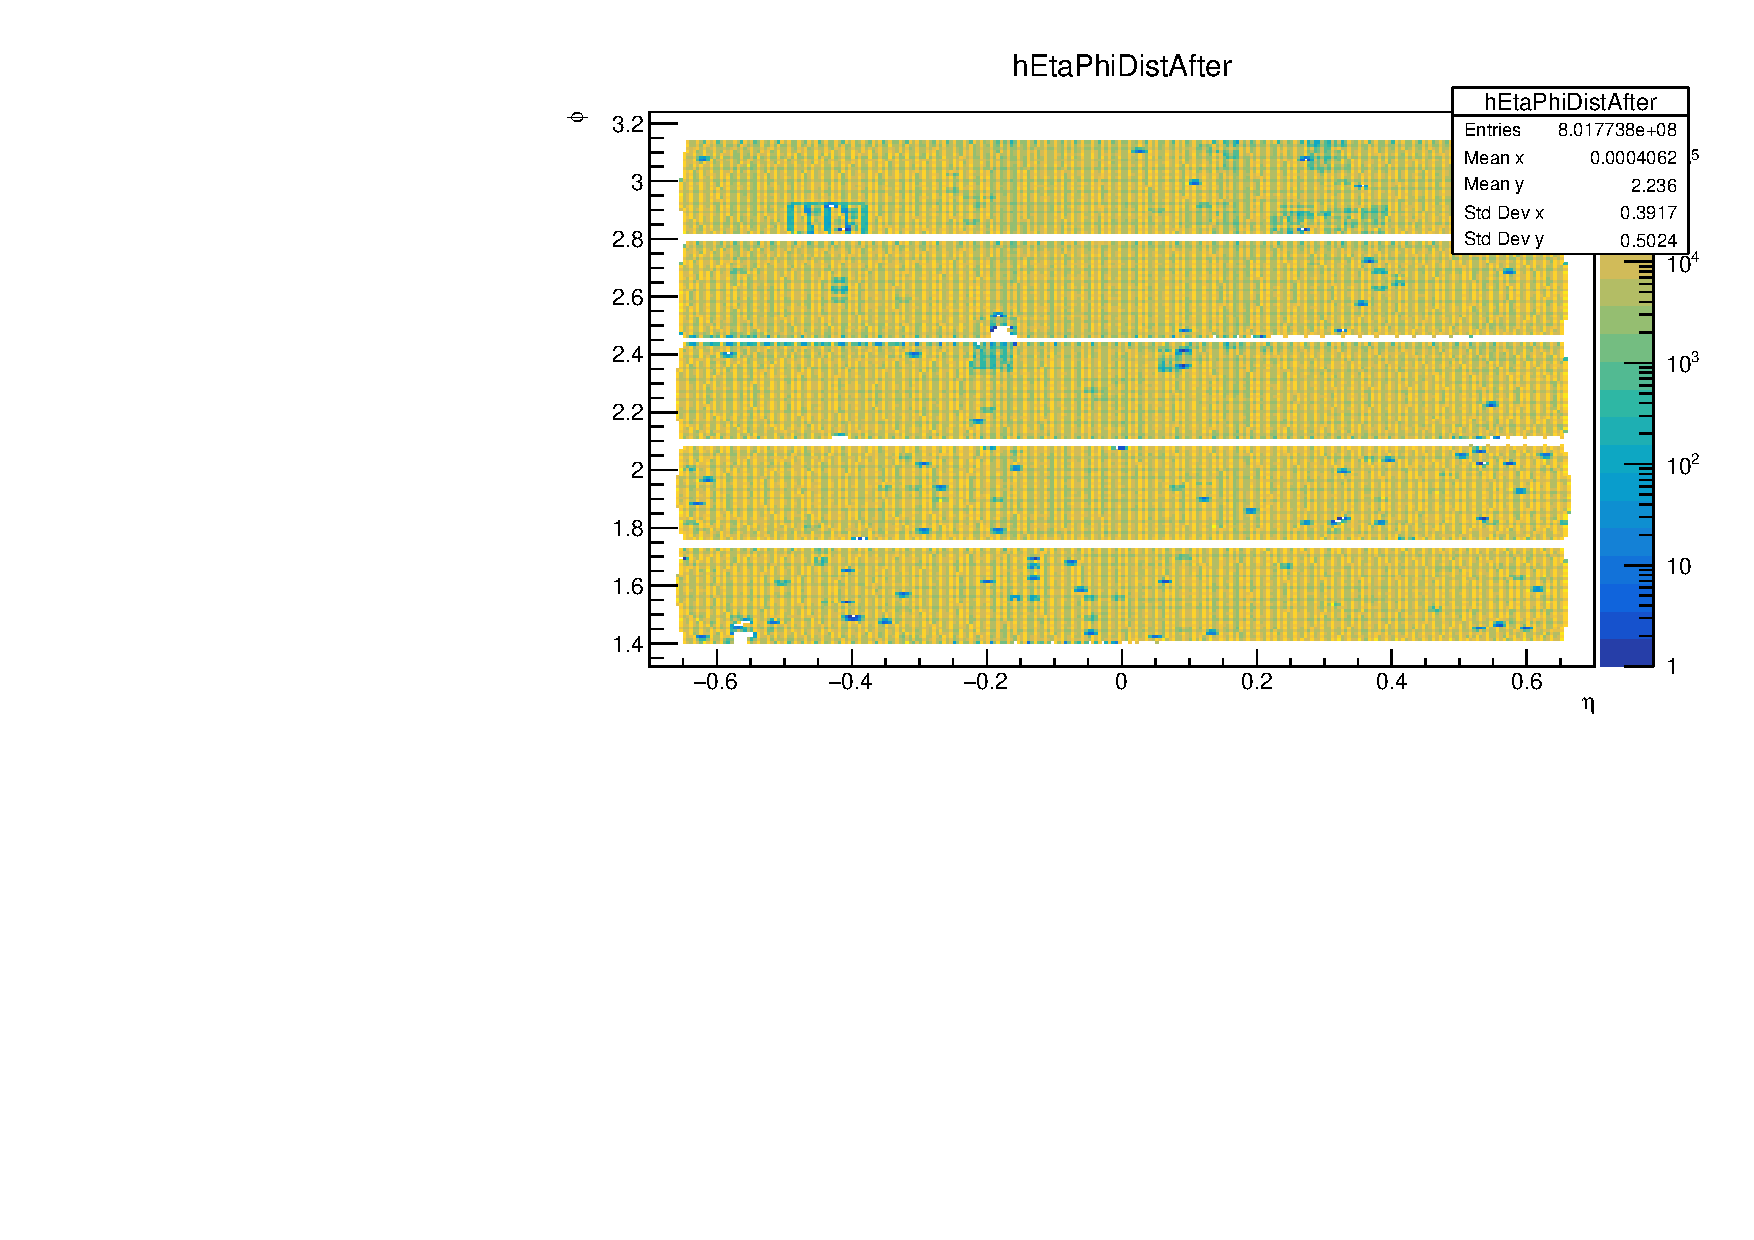
\includegraphics[width=14cm]{BadChannelMap}
\centering
\caption{EMCal cell occupancy after bad channels removed.}
\label{fig:badchannel}
\end{figure}

After these corrections were applied, the towers were grouped together into clusters using a clustering algorithm.  The algorithm finds any EMCal tower with minimum tower energy of 300 MeV and uses this as a seed, after which all adjacent towers with a minimum energy, $E_{cell} \geq \,$ 100 MeV, are iteratively added using a method similar to the $k_{T}$ algorithm from Chapter \ref{ch:qcd}.  After this point the set of clusters for a given event have been reconstructed.  The cluster energy is the sum of the seed tower and grouped neighbor tower energies.  EMCal clusters are corrected for exotics.  This correction was performed by cutting all clusters with a $F_{cross} \geq \,$ 0.97, where

\begin{equation}
F_{cross} = 1 - \frac{ E_{cross} }{ E_{cell} },
\label{eq:Fcross}
\end{equation}

\noindent
where $E_{cross}$ is the sum of the four cells sharing a full edge with the leading cell and $E_{cell}$ is the center pixels energy.  The main source of exotic clusters in the EMCal is most often due to a hadron hitting the Avalanche Photodiode (APD) in a tower.  This will concentrate the energy of the cluster into a single tower while the adjacent towers will contain only a small fraction of the cluster energy.  The exotic clusters were removed before jet finding occurred as they are an artifact of the detector performance.

The EMCal is optimized to measure neutral particles, photons and neutral pions as they will fully shower inside of the sub-detector.  Hadrons are detected by the EMCal, but will only shower a fraction of their intrinsic energy.  A hadronic correction was performed in order to account for double counting as charged hadrons will depsit energy in both the TPC and EMCal.  To identify charged hadrons, charged tracks from the outer layer of the TPC were propagated to the EMCal, by fitting the trajectory of the track to a curve, and fitting the tracks and clusters geometrically.  Figure \ref{fig:EMChadetaphi} shows the distance between the centroid of a cluster in the EMCal and the nearest track propagated from the TPC.  Hadrons are identified by requiring the matched distance to be, $\sqrt{ \Delta\phi^{2} + \Delta\eta^{2} } \leq \,$ 0.015, which is within one EMCal tower distance.  A non-linear correction to the cluster energy is applied based on the 2010 test beam data to account for the non-uniform energy response.

\begin{figure}[h]
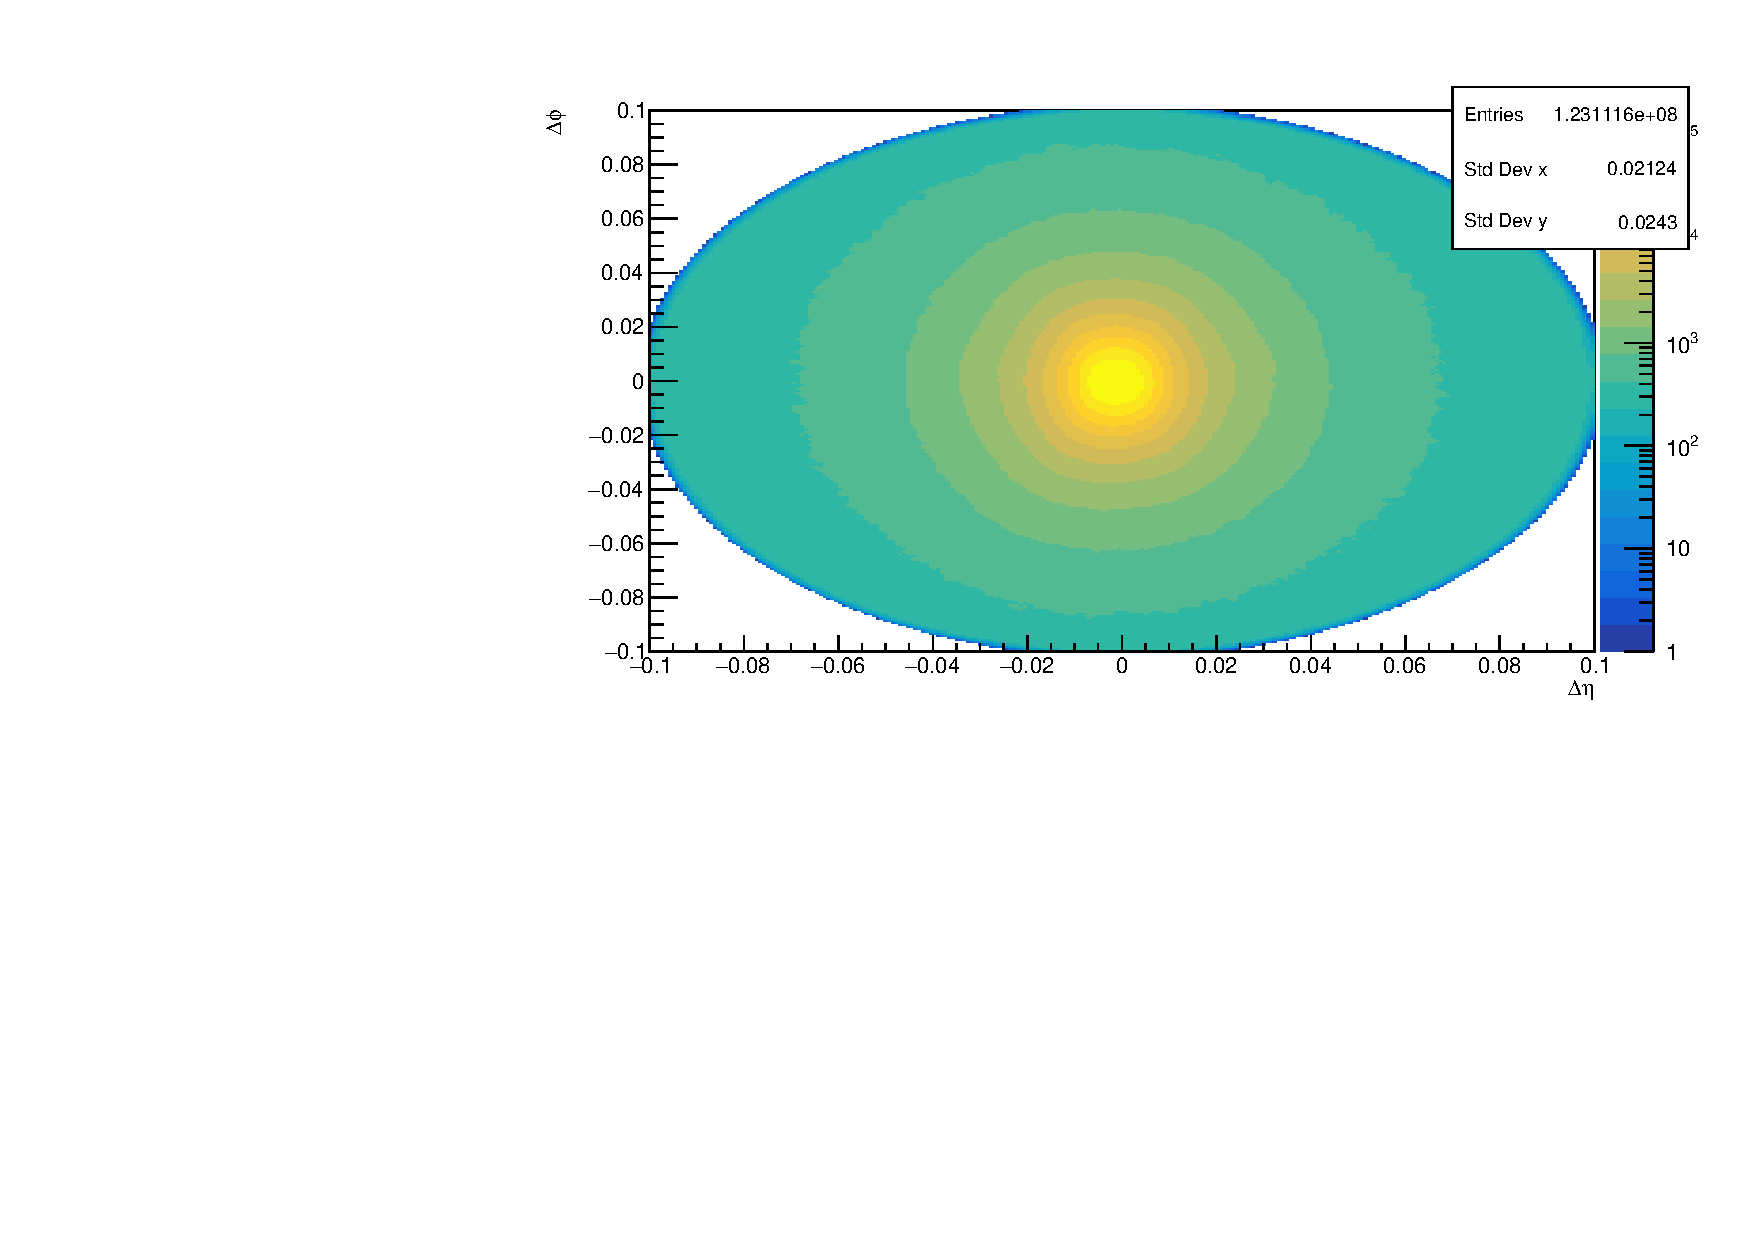
\includegraphics[width=12cm]{hadronetaphi}
\centering
\caption{Matched track-cluster distance.}
\label{fig:EMChadetaphi}
\end{figure}


Corrections for the double counting from hadrons is based on correcting the EMCal cluster energy by a weight function

\begin{equation}
E_{corr} = E_{clust} - f_{sub} \times \sum p ,
\label{eq:HadCorr}
\end{equation}

\noindent
where $\sum p$ is the magnitude of the 3-momentum of the hadron and $f_{sub} = 1$ is the nominal value for the weight.  If $E_{corr} \leq 0$ the cluster was removed.  This may be caused by cluster pile-up and only accounted for a small fraction of the clusters.  In order for a cluster to be accepted $E_{corr} \geq \,$ 300 MeV was required, because a minimum ionizing particle (MIP) will on average deposit 280 MeV in the EMCal.  

A final cut was performed on the cluster timing, obtained from the T0, the time of arrival for a particle is shown on the y-axis of Figure \ref{fig:EMCaltime}.  

\begin{figure}[!h]
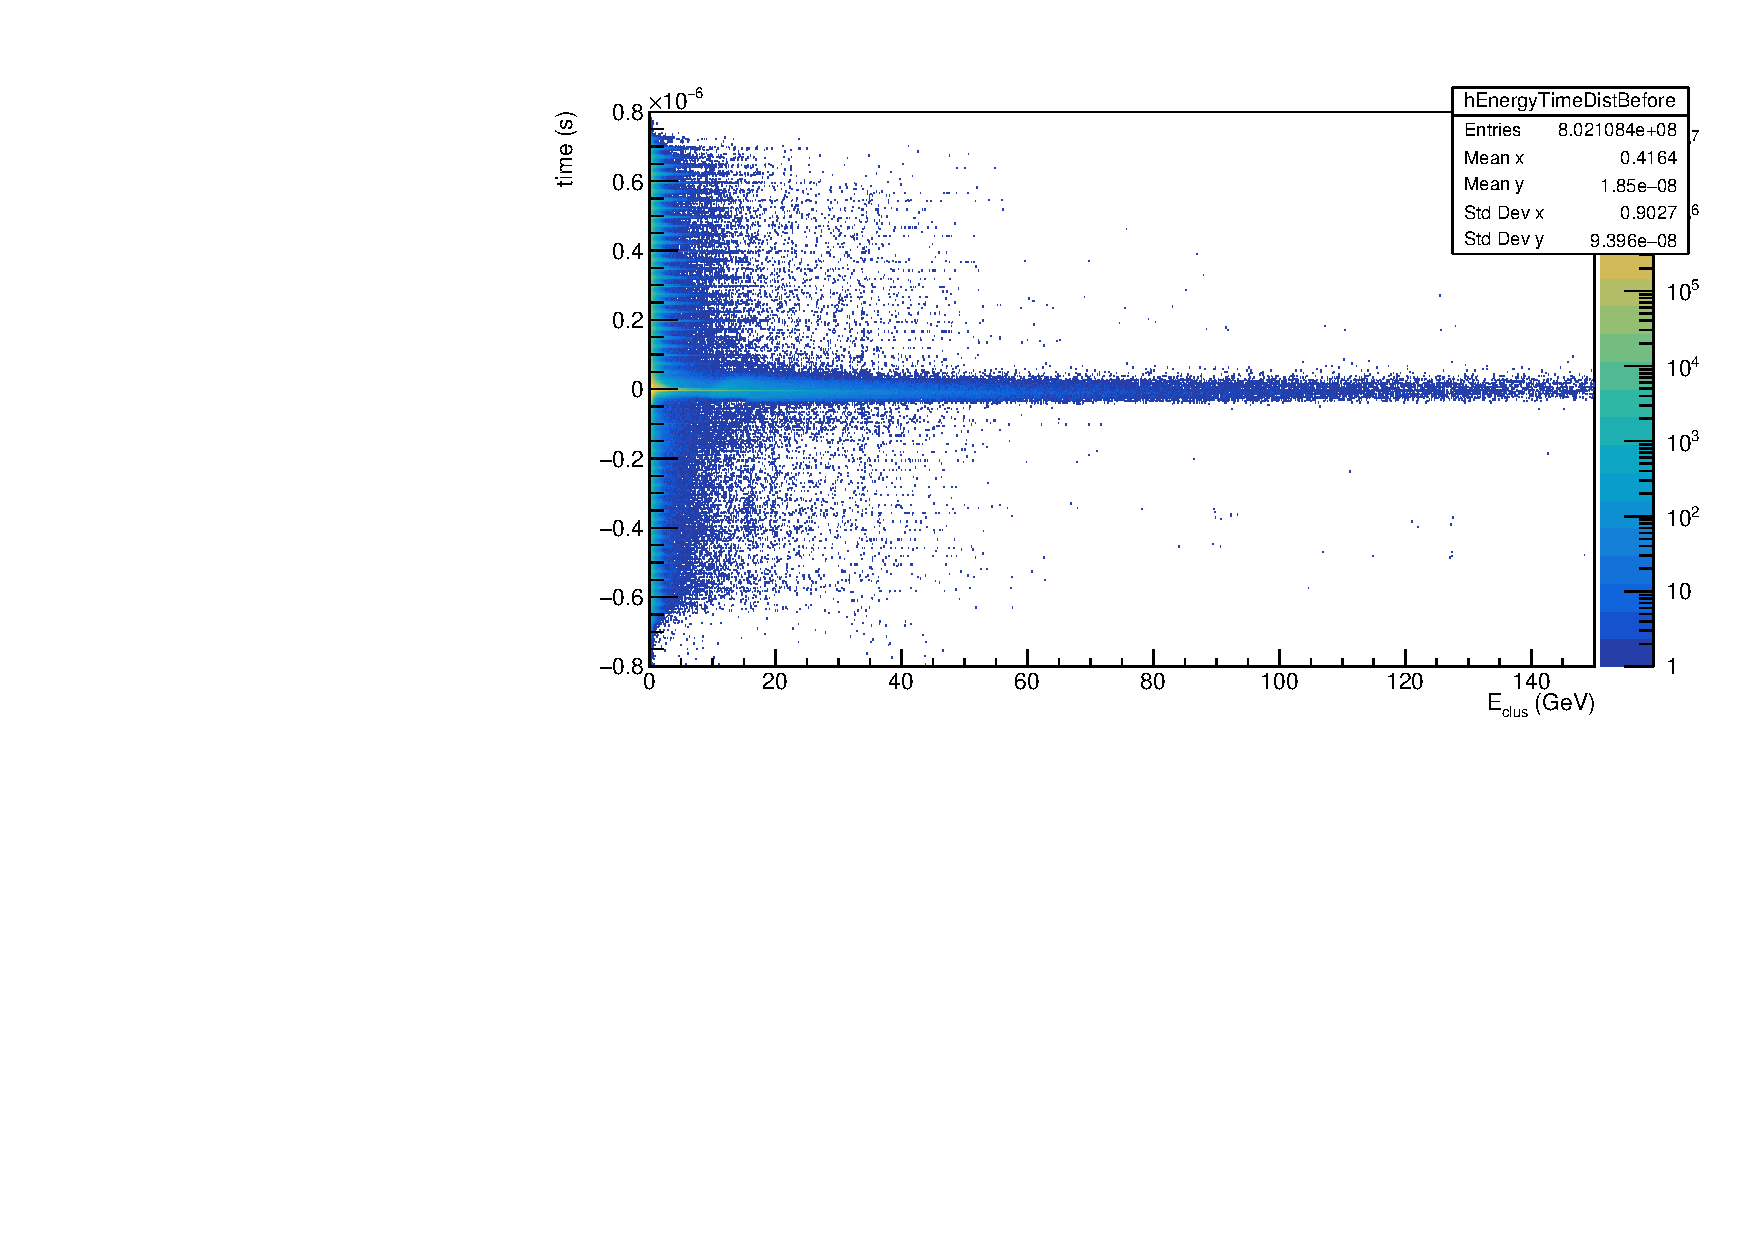
\includegraphics[width=11cm]{timming}
\centering
\caption{EMCal cluster time distribution before cuts.}
\label{fig:EMCaltime}
\end{figure}


Cutting on the cluster time is done in order to readout only the particles created from an event and to limit the contamination due to slower particles from previous events.  The main source of the slow moving particles are `slow' neutrons and $K_{L}^{0}$ from the previous collision or detector noise, this analysis limited cluster time to $t_{clus} \, \epsilon \,$ [-50 ns, 100 ns].


\begin{figure}[h]
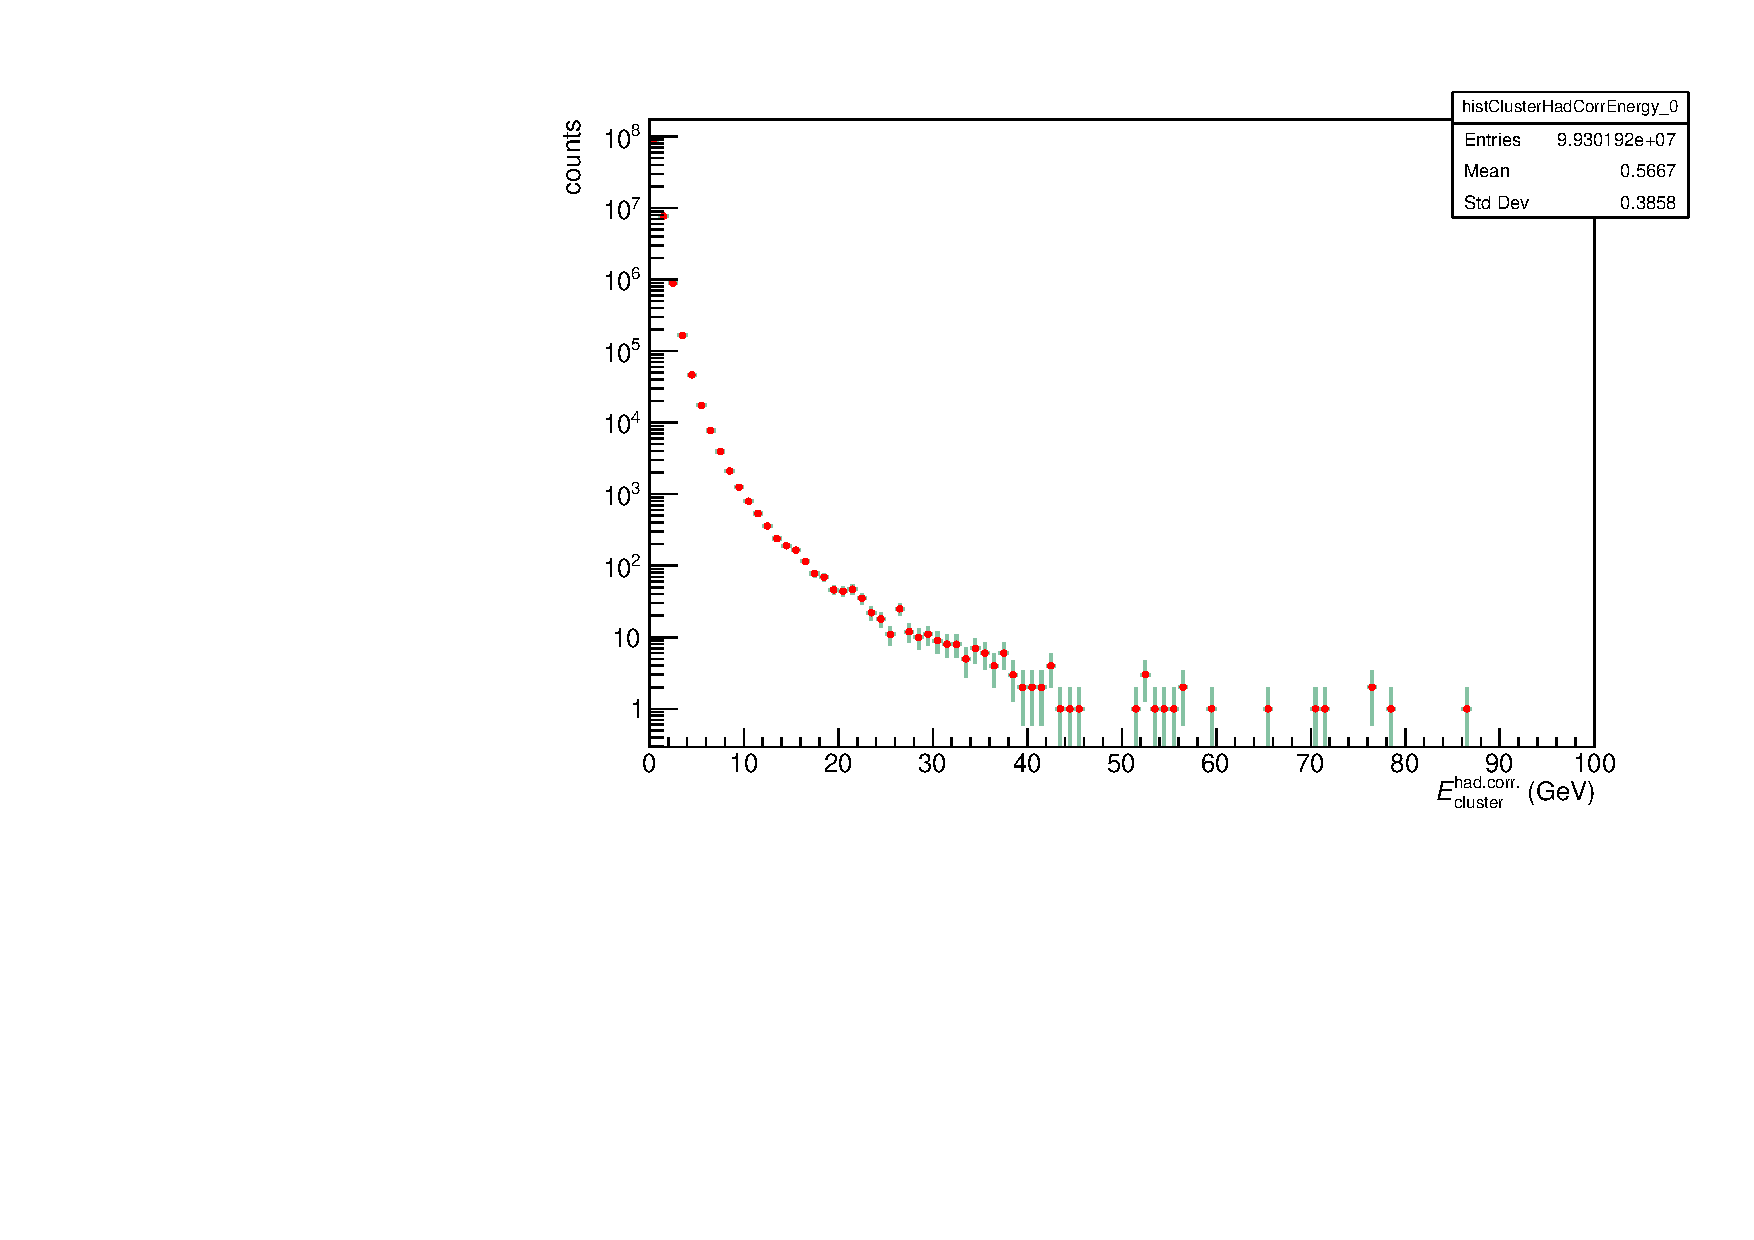
\includegraphics[width=8cm]{Eclusfinal}
\centering
\caption{Corrected EMCal cluster yield.}
\label{fig:EMCalfinal}
\end{figure}
\newpage

Figure \ref{fig:EMCalfinal} shows the final cluster energy distribution with all the cuts and corrections.  The same cuts and corrections were applied to the EMCal triggered data.  Clusters with an energy greater than 300 MeV were used for the jet finding due to the uncertainty in the energy response of the EMCal

\section{TPC Tracks}

Tracks were reconstructed in the TPC using a Kalman filter which helps alleviate any corrections needed due to multiple scatterings, dead sectors, energy loss, etc.  The Kalman filter used in ALICE reconstructs tracks using the following approach.  First, the algorithm finds hits on the outer radius of the TPC where the track density is the lowest.  For each of these track candidates the algorithm starts to reconstruct the track by adding hits from the TPC as it's traced inward from the TPC radius.   Once all the hits are reconstructed into tracks on the inner radius of the TPC, ITS track reconstruction takes over and the track is traced back to the primary vertex as best as possible.  If the track reconstruction was successful a second pass begins, this time starting from the primary vertex, moving through the ITS, and finishes at the outer wall of the TPC.  Track candidates that are successfully reconstructed during both of the passes go through a third and final reconstruction starting from the outer wall of the TPC moving backwards towards the vertex region.  Once the three passes are complete the track parameters are finalized and the tracks from the event are recorded. 
Tracks can have a number of inefficiencies and non-uniformities present in them.  Using `hybrid' tracks helps with non-uniformities and ensures that tracks have a uniform distribution in the detector.  Hybrid tracks consist of two track sets, the first being all tracks with at least one hit in the SPD (Global), and the second set being all tracks that can be constrained to the primary vertex (Complimentary).  By using complimentary tracks for jet finding we ensured good $p_{T}$ measurement because the track traversed a large portion of the TPC.  

The reconstruction of a signal from the ITS and TPC form good tracks if the $\chi^{2}/NDF$, chi-square per degrees of freedom, is required to be less than 4 in the TPC and $\chi^{2}$ is required to be less than 36 in the ITS. For this analysis, the minimal $p_{T, track}$ was 150 MeV/c and the track was constrained to the acceptance: - 0.9 $\leq \eta \leq$ 0.9 and 0 $\leq \phi \leq$ 2$\pi$, shown in Figure \ref{fig:Hybridtracketaphi}. Tracks were further constrained by forcing them to have a distance of closest approach to the primary vertex of less than 2.5 cm in the plane transverse to the beam line and less than 3.0 cm along the beam axis.  The spatial distributions of the hybrid tracks remain relatively flat as expected in the 8 TeV data set for good and semi-good runs.

\begin{figure}%
    \centering
    \subfloat[Hybrid Track $\eta$]{{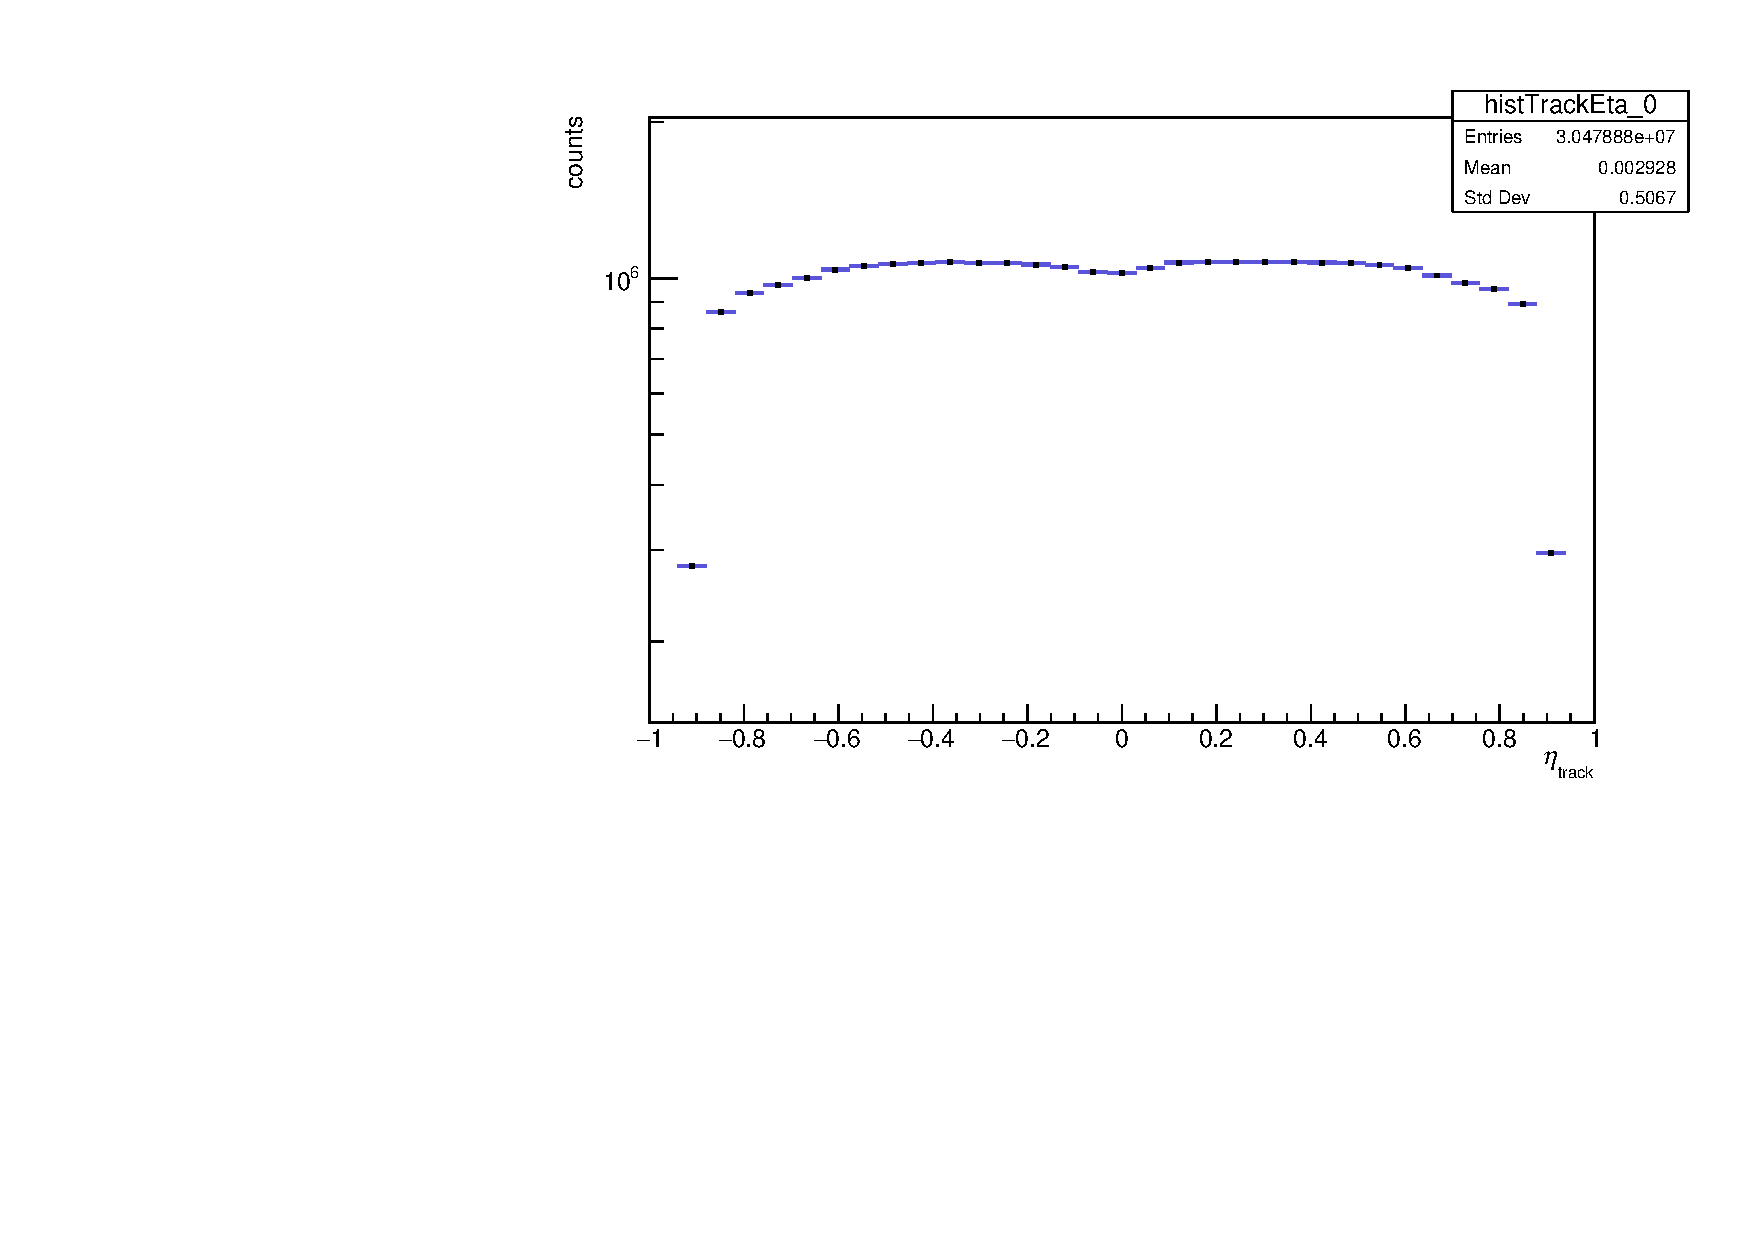
\includegraphics[width=0.5\textwidth]{tracketa} }}%
    \qquad
    \subfloat[Hybrid Track $\phi$]{{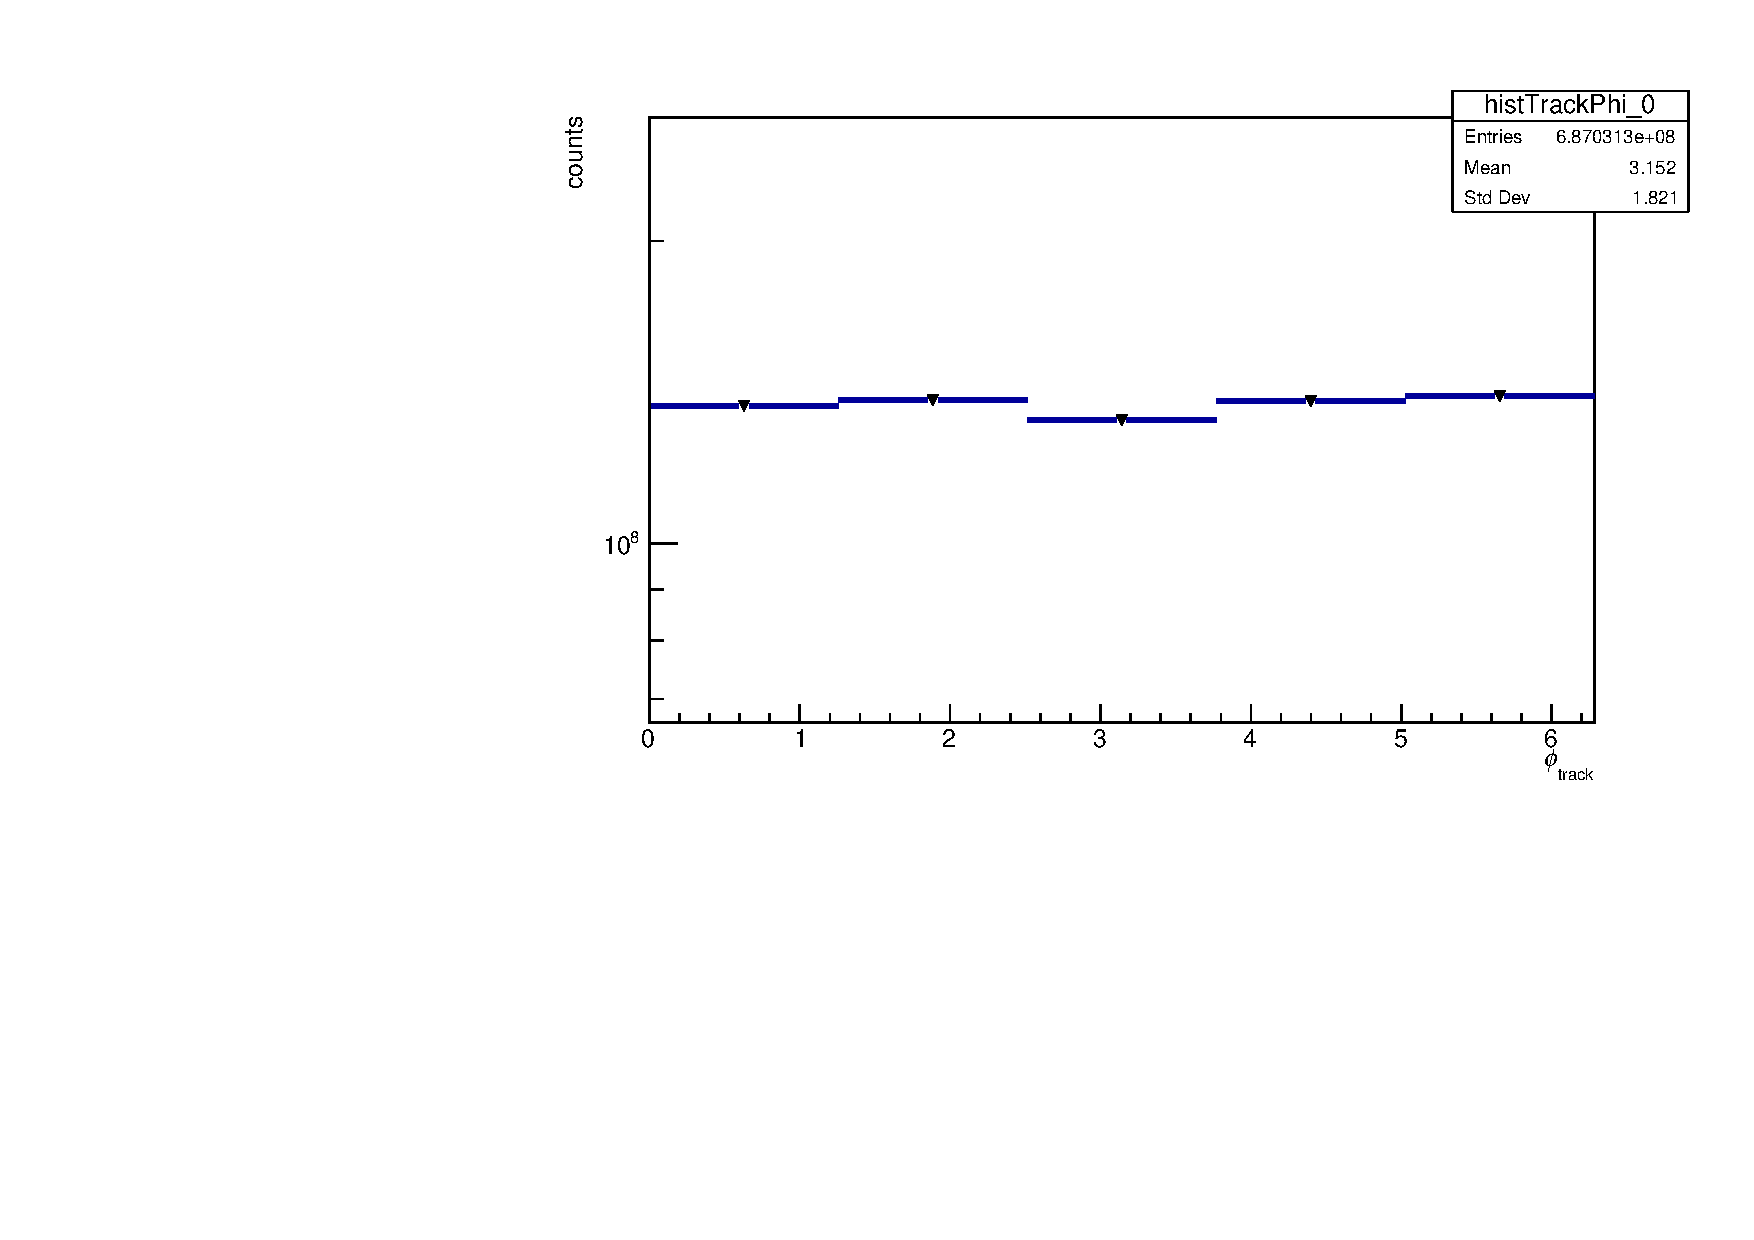
\includegraphics[width=0.5\textwidth]{trackphi} }}%
    \caption{Hybrid Track $\eta$ and $\phi$ yields.}%
    \label{fig:Hybridtracketaphi}%
\end{figure}


An important parameter of the hybrid track is the track $p_{T}$ resolution which determines how well the track momentum was measured.  The quality of the jet $p_{T}$ resolution was maintained by only accepting tracks into the jet finder with a resolution below 1\% as seen in Figure \ref{fig:trackresolution}, which was obtained by varying the parameters from the kalman fit.  The accepted complimentary track $p_{T}$ distribution may be seen in Figure \ref{fig:hybtrackpt}.  Tracks should travel in a smooth curve unless they decay in the detector.  Tracks in the TPC may exhibit a kink due to the particle decays or misreconstructions.  Tracks with a kink were excluded from this analysis.  The track quality control used in this thesis followed previous ALICE jet results\cite{Acharya:2018eat}.  The cuts and quality control were used uniformally for tracks from Min Bias events and from the EMCal triggered data.

\begin{figure}[h]
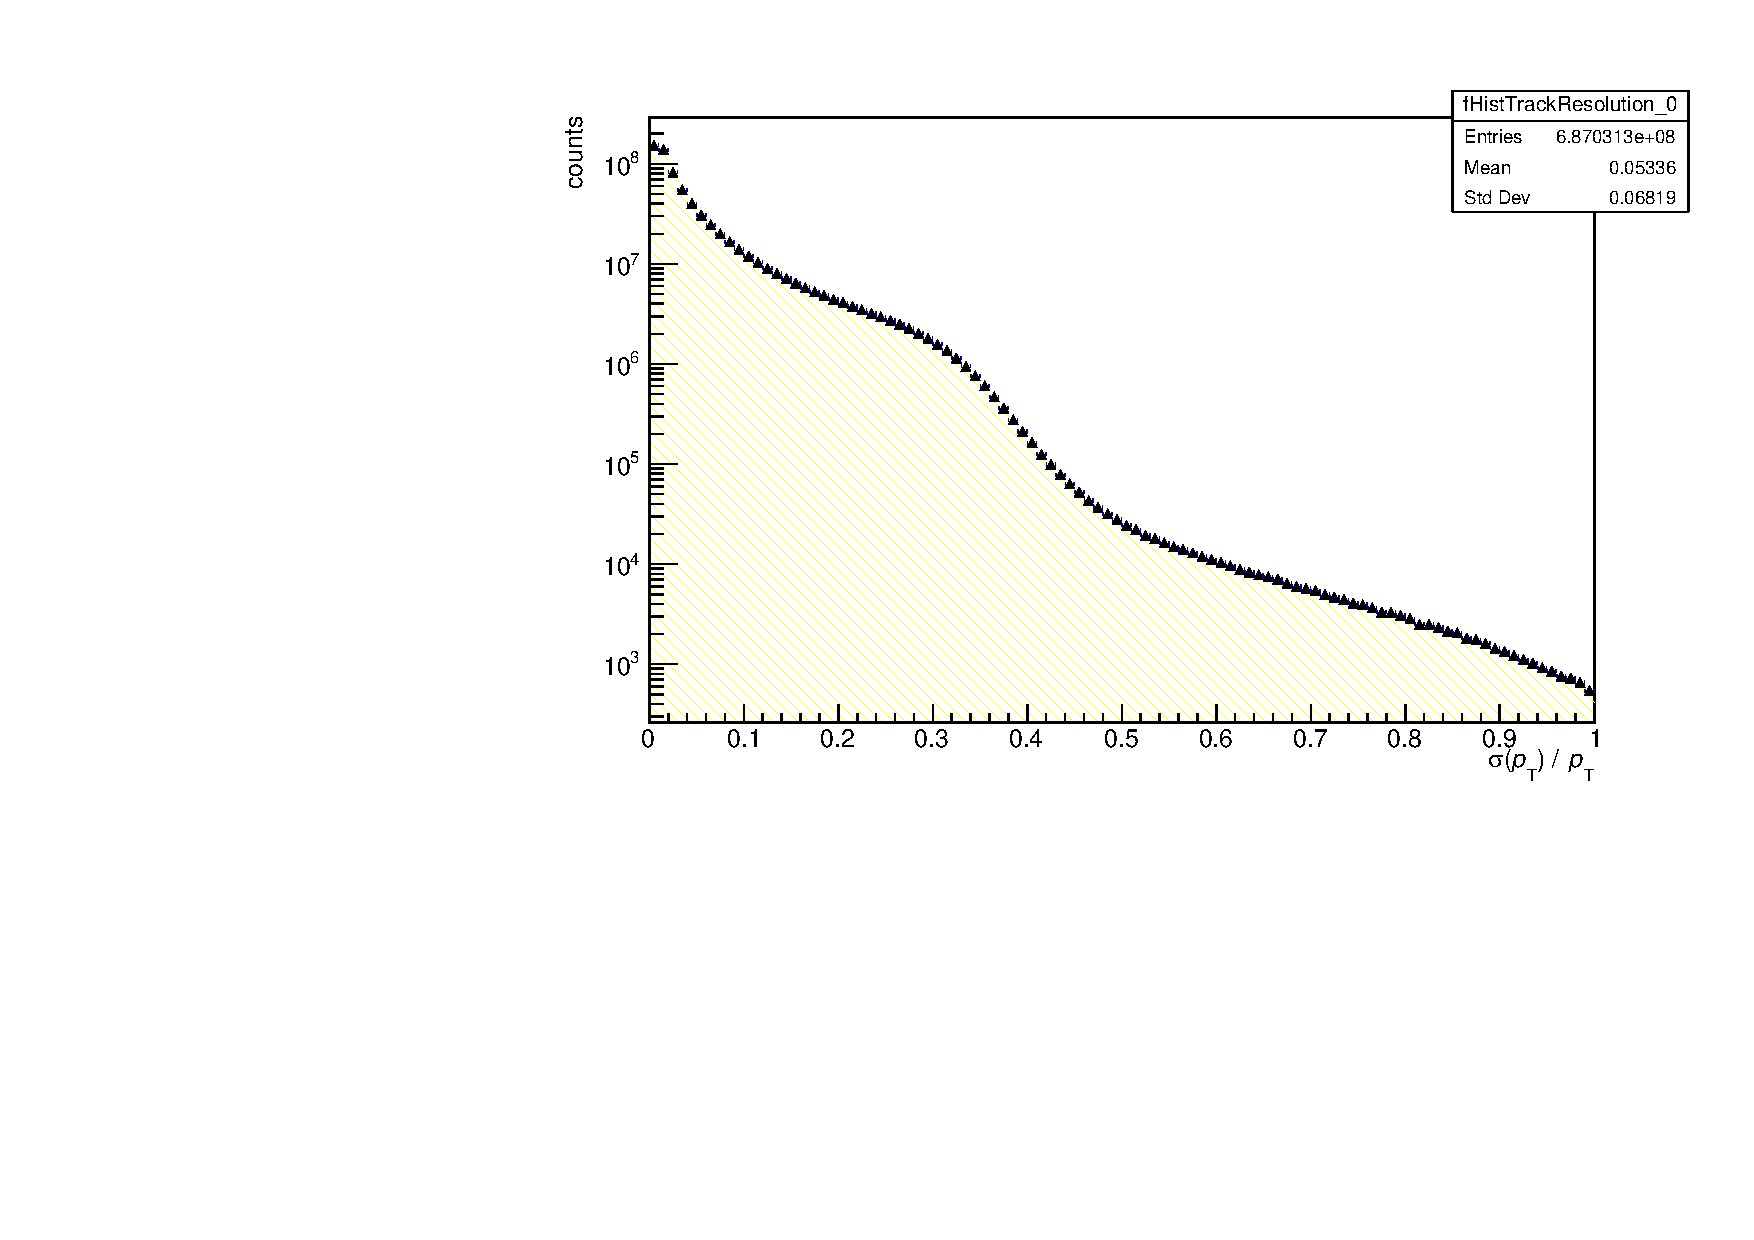
\includegraphics[width=8cm]{trackresolution}
\centering
\caption{Accepted hybrid track resolution.}
\label{fig:trackresolution}
\end{figure}

\begin{figure}[h]
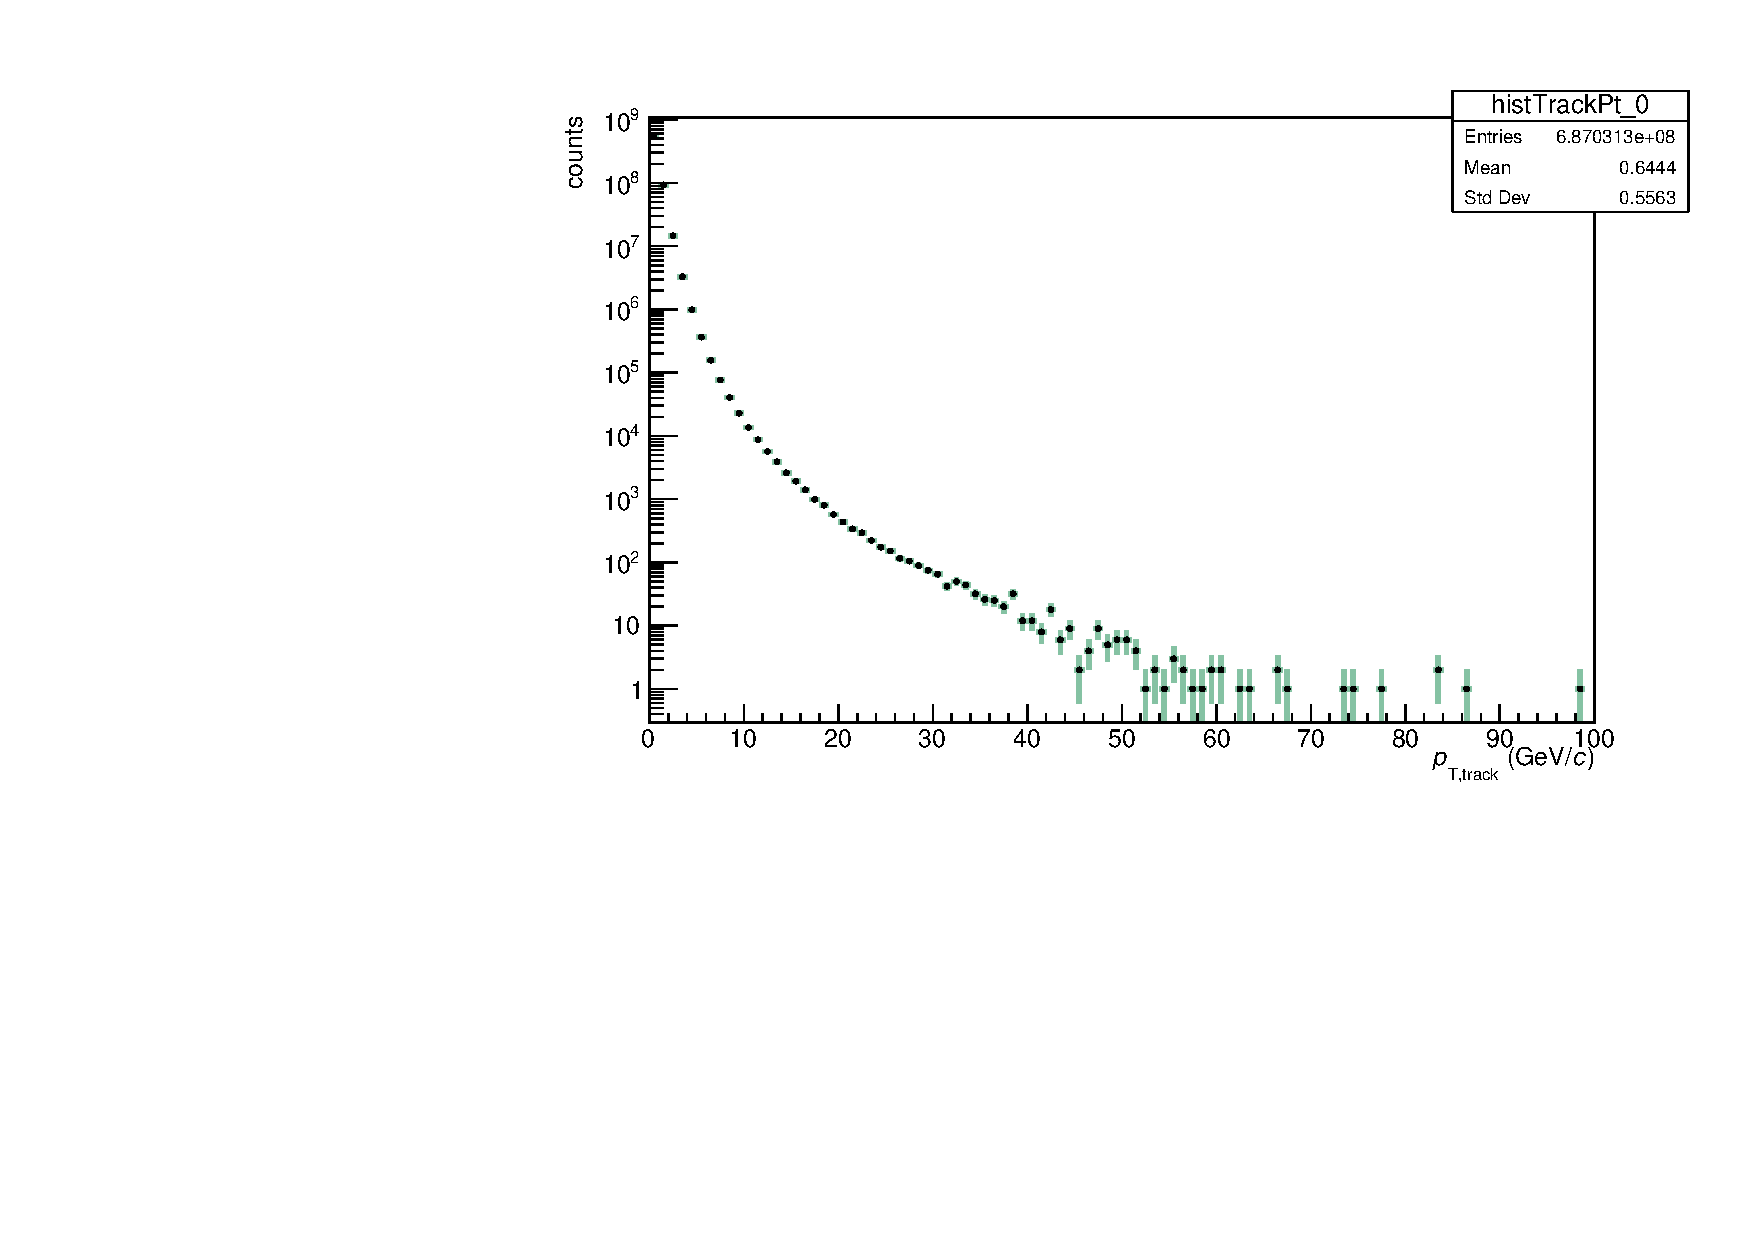
\includegraphics[width=8cm]{trackpt}
\centering
\caption{Accepted track $p_{T}$ yield.}
\label{fig:hybtrackpt}
\end{figure}


\section{Raw Jet Reconstruction}

Tracks and clusters that passed the QA requirements were used for anti-kt jet reconstruction to measure inclusive jets.  A minimum threshold of 5 GeV was used to reconstruct a jet in this analysis because of ambiguities in the QCD definition jet below this range.  This analysis used the p-scheme recombination method discussed in Chapter 2. No tracks above 100 GeV/\textit{c} were used in the jet finding due to the tracking resolution, Figure \ref{fig:JetPt} shows the distribution of the track momentum for a given jet momentum.  In addition a cut was applied that a jet must be composed of at least two constituents, as shown in Figure\ref{fig:JetConst}.

 \afterpage{%
\begin{figure}[h]
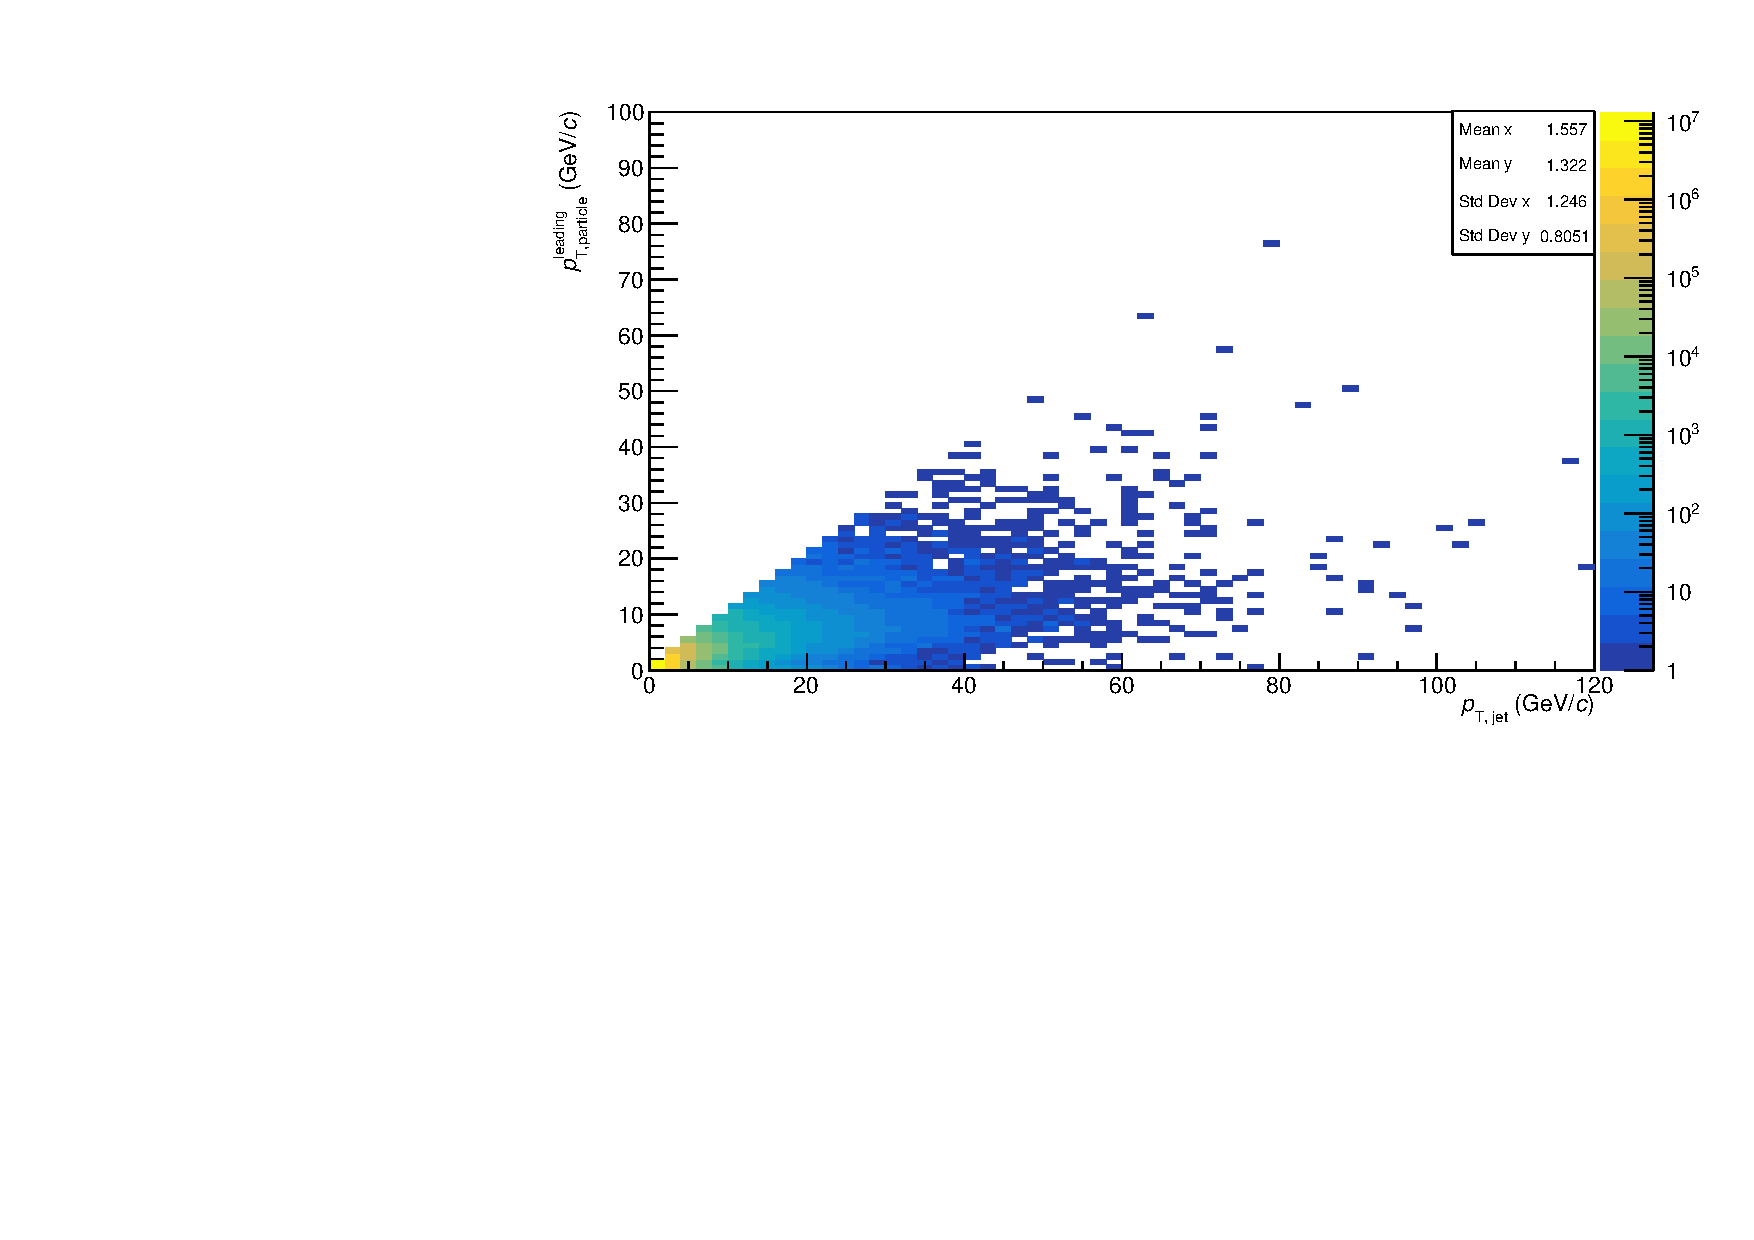
\includegraphics[width=\linewidth]{ptleadingR02}
\centering
\caption{R = 0.2 leading track $p_{T}$ per jet $p_{T}$.}
\label{fig:JetPt}
\end{figure}

\begin{figure}[h]
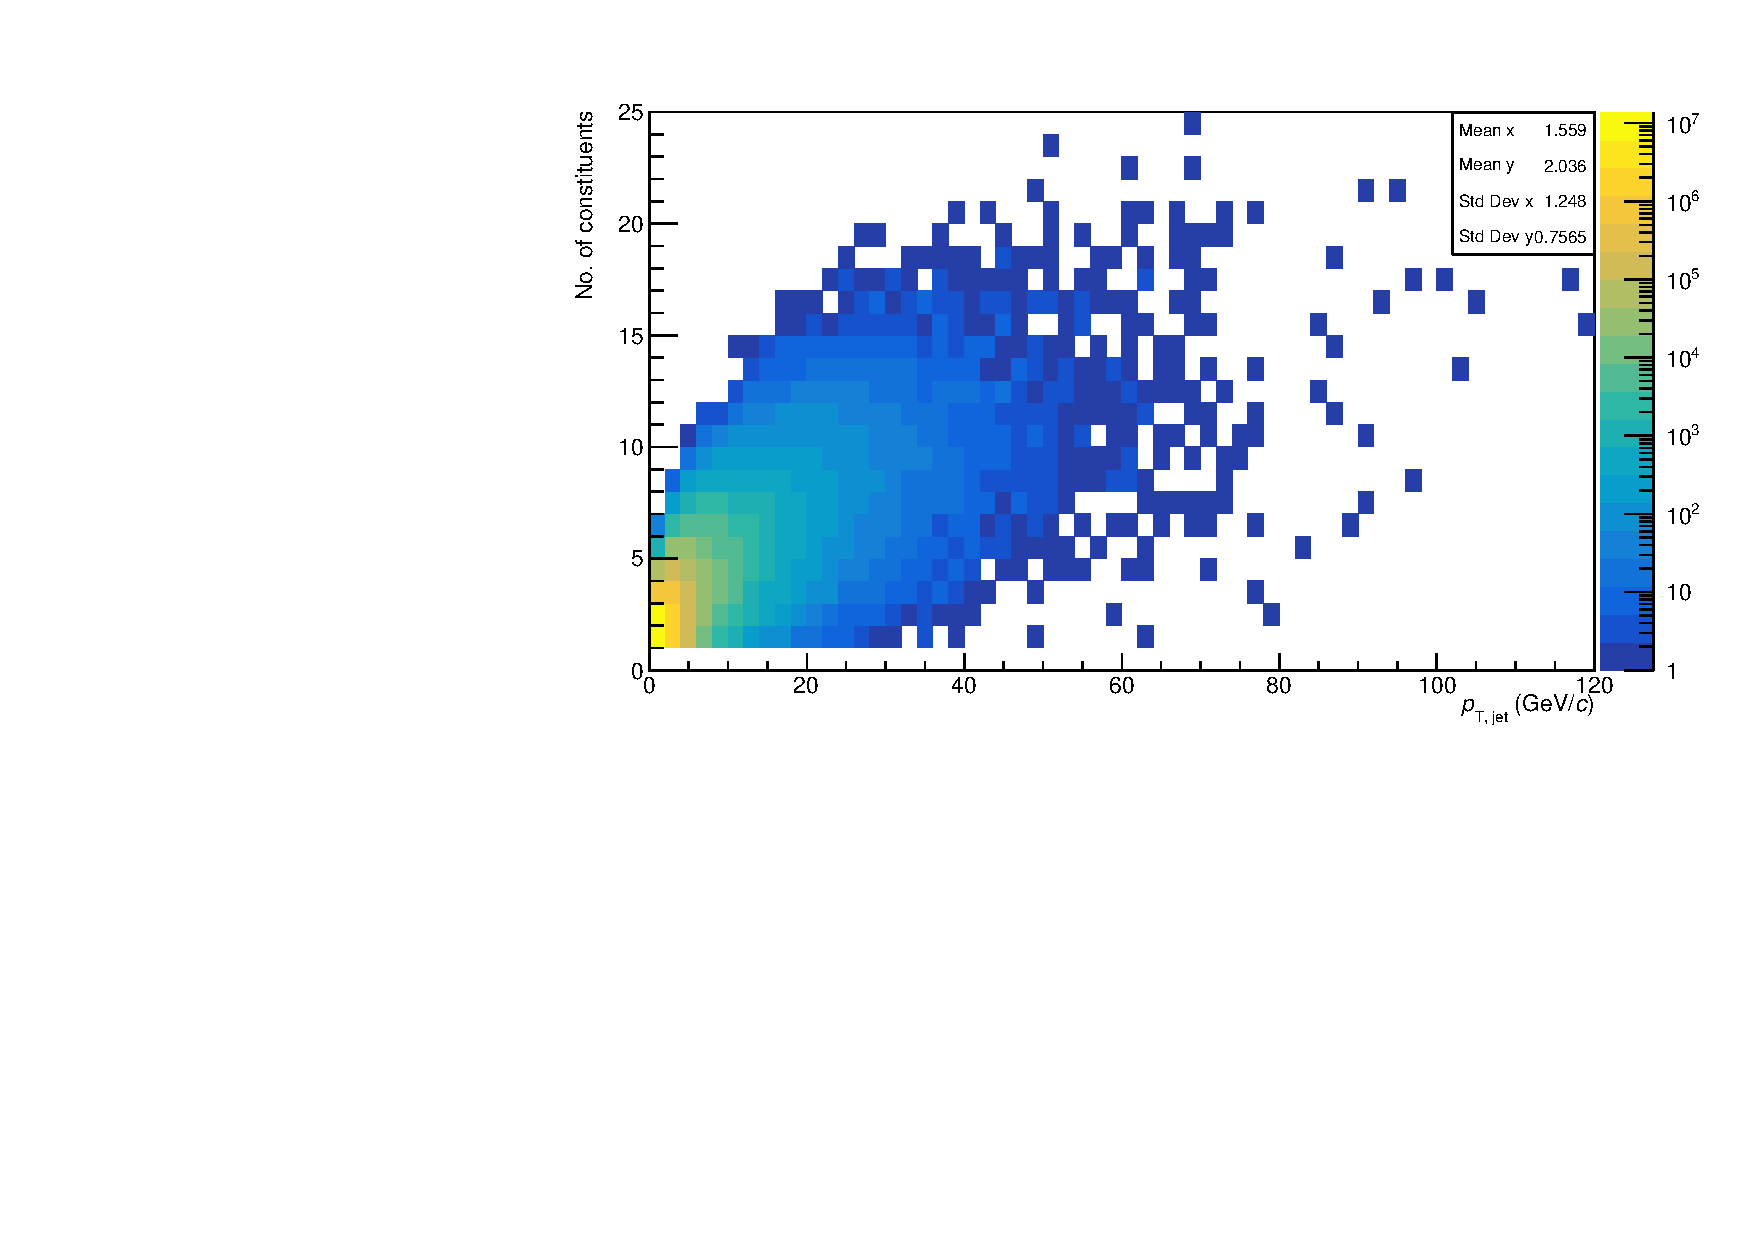
\includegraphics[width=\linewidth]{JetnumcconstR02}
\centering
\caption{R = 0.2 number of constituents in a jet per jet $p_{T}$.}
\label{fig:JetConst}
\end{figure}
\clearpage
}

The z for the leading track,

\begin{equation}
z_{leading} = \frac{ p_{leading, proj} }{ p_{jet} },
\label{eq:zleading}
\end{equation}

\noindent
may be artificially high due to misidentifying secondary decay particles as primary vertex tracks and assigning them a much larger $p_{T}$.  Additionally, fake clusters, such as exotics, may skew the $z_{leading}$ quantity.  

\begin{figure}[h]
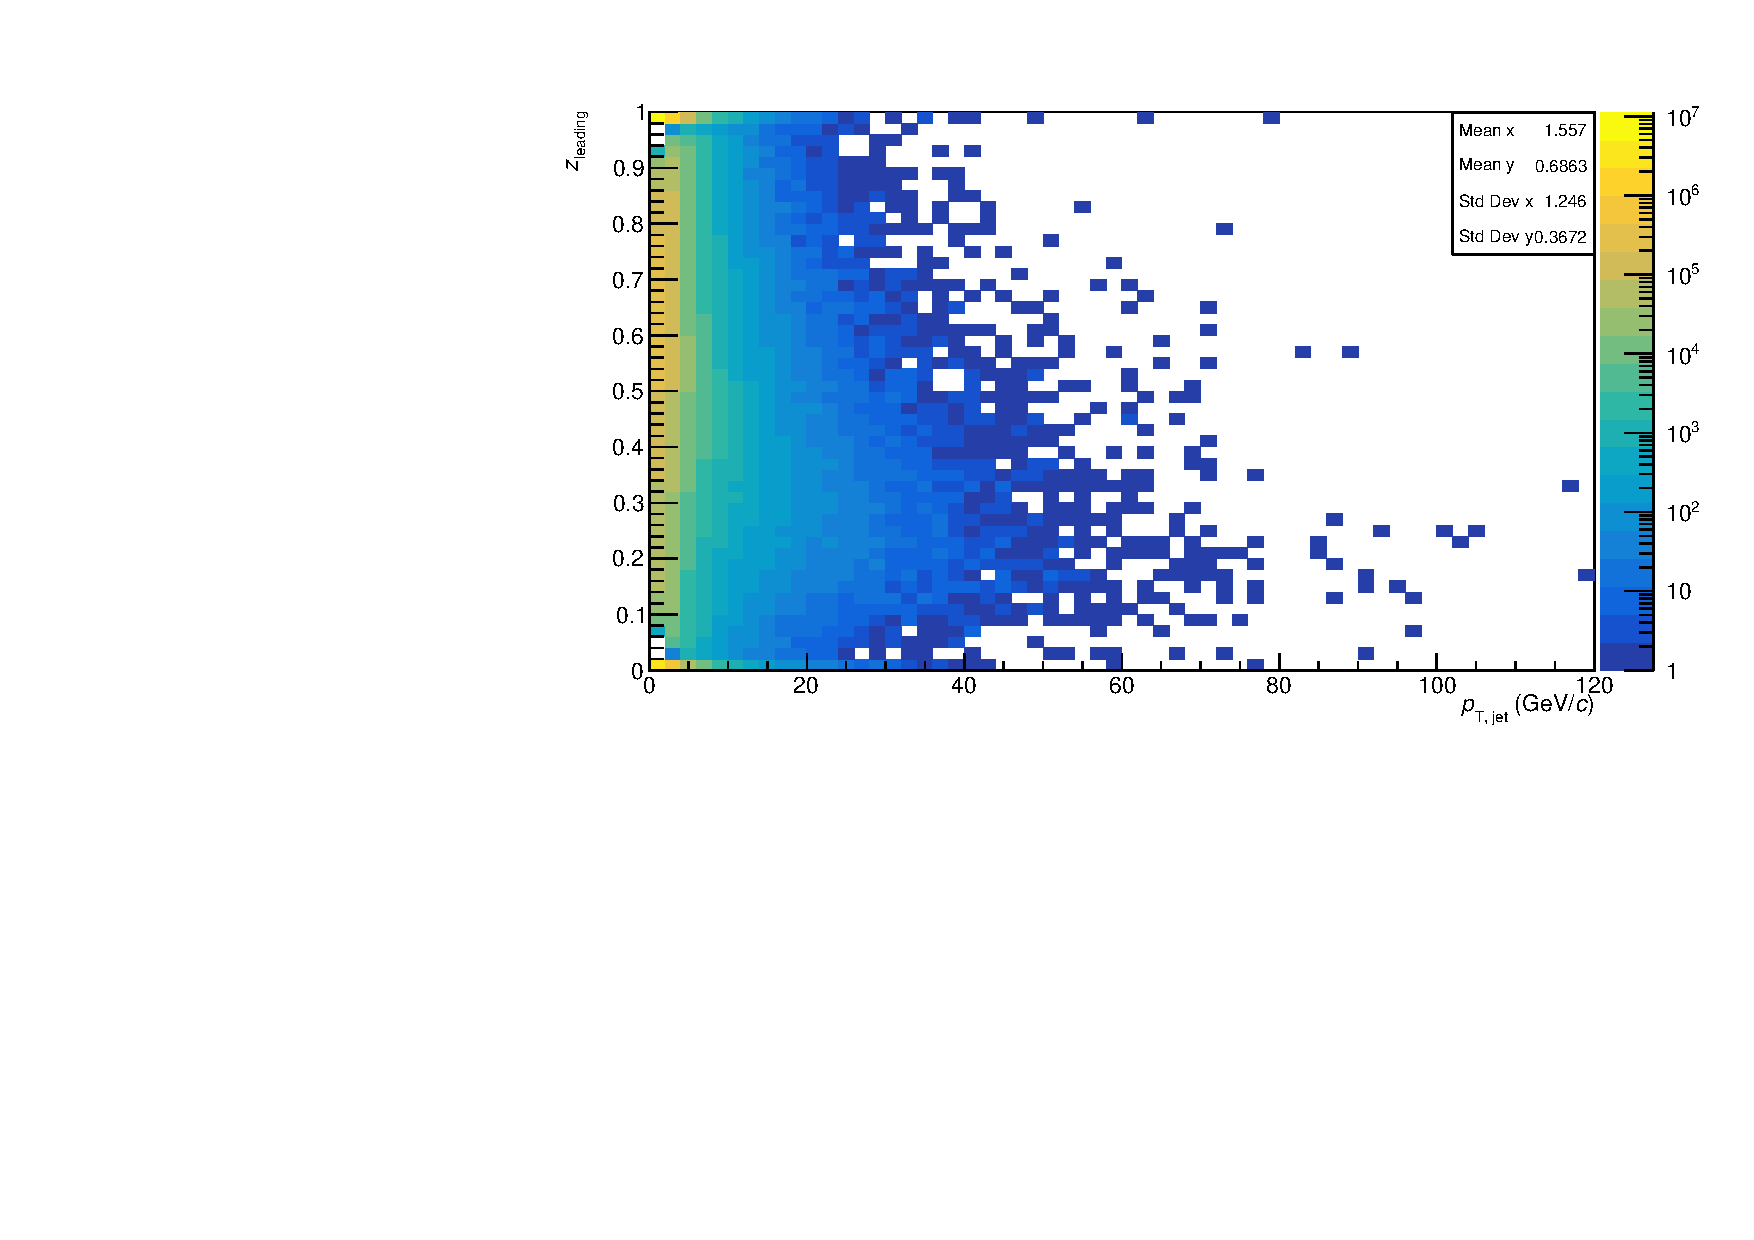
\includegraphics[width=10cm]{JetzR02}
\centering
\caption{R = 0.2 $z_{leading}$ from the Min Bias data sample.}
\label{fig:Jetz}
\end{figure}

z_{leading} was investigated during this analysis. Figure \ref{fig:Jetz} shows the $z_{leading}$ for a given jet $p_{T}$.  We observed an excess of jets, especially at low jet $p_{T}$, of $z_{leading}$ values close to 1 or zero.  Previous jet results from ALICE removed these jets with a cut on $ z_{leading} \geq 0.03$ and $z_{leading} \leq 0.97$ in order to exclude tracks created from low energy daughter decays and noisy towers from the EMCal.  However, a $z_{leading} \sim 1$ corresponds to a jet dominated by a singular high-$p_{T}$ particle.  Although unlikely this is allowed by QCD and thus no $z_{leading}$ cut was implemented in this analysis.  In between .03 and .97 we see the $z_{leading}$ is continuous and uniform as expected.  

A jet area of, $A_{jet}$, cut was imposed on accepted jets.

\begin{equation}
A_{jet} \geq 0.6 \pi R_{jet}^{2}
\label{eq:AreaJet}
\end{equation}

\noindent
The area is estimated in FastJet using `ghost' particles.  As jet reconstruction is being performed, these fake particles with infinitesimal $p_{T}$ are placed randomly throughout the event.  The number of ghost particles captured in a jet is proportional to the jet area, thus the precision of the jet area is sensitive to the reconstruction of soft particles.  Jet area cuts are atypical in a proton-proton analysis, however one is implemented in this thesis so that the final jet cross-sections can serve as a baseline measurement for heavy-ion jet measurements.

Figure \ref{fig:jetRejection} shows the rejection reason for a jet from the 8 TeV data, the dominate reason for cutting a jet was due to the area criteria this cut skewed towards low-$p_{T}$ jets.  Jet area cuts are atypical in proton-proton measurements.  Due to the high multiplicity environment present in heavy-ion collisions area cuts are much more common, by using an area cut the jet results presented in this thesis better serve as a baseline measurement for jet quenching.

\begin{figure}[h]
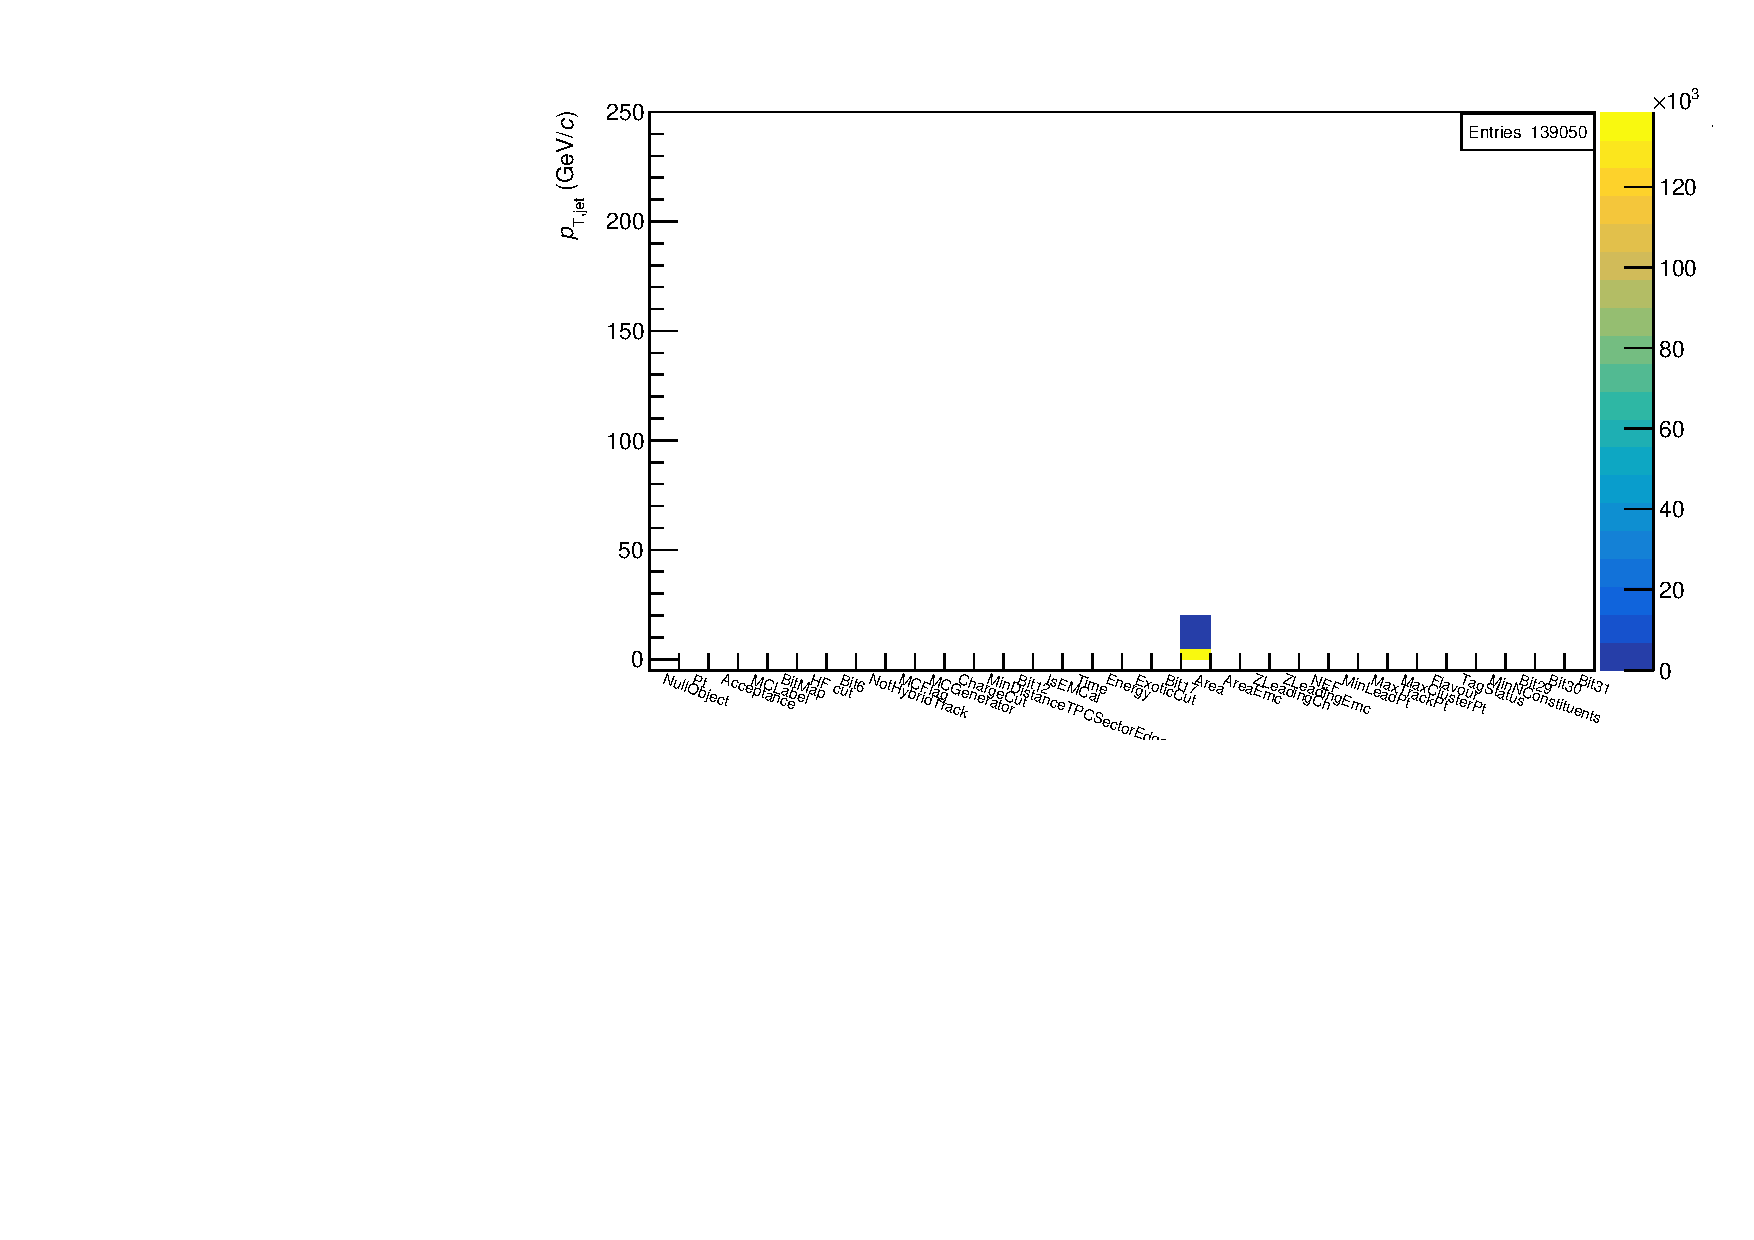
\includegraphics[width=12cm]{jetRejection}
\centering
\caption{Jet rejection reason.}
\label{fig:jetRejection}
\end{figure}


The Neutral Energy Fraction (NEF) is the total jet energy carried by the neutral components of the jet, i.e. EMCal clusters.  Figure \ref{fig:JetNEF} shows the NEF for R = 0.2 jets from the Min Bias sample.

The 8 TeV data was investigated and we observed an excess of jets at low-$p_{T}$ with NEF values around zero or one, similar to what was seen with the $z_{leading}$ distribution.  The cause for these excesses were explored in this analysis, but no hard source was identified and no cut to the NEF was used.  Previous ALICE jet results cut the low and high range of the of the NEF, but from the QCD standpoint these jets are allowed.  No NEF cut was implemented for this analysis.

The criteria and cuts discussed were implemented for the R = 0.3 and R = 0.4 along with the EMCal triggered data.

\begin{figure}[h]
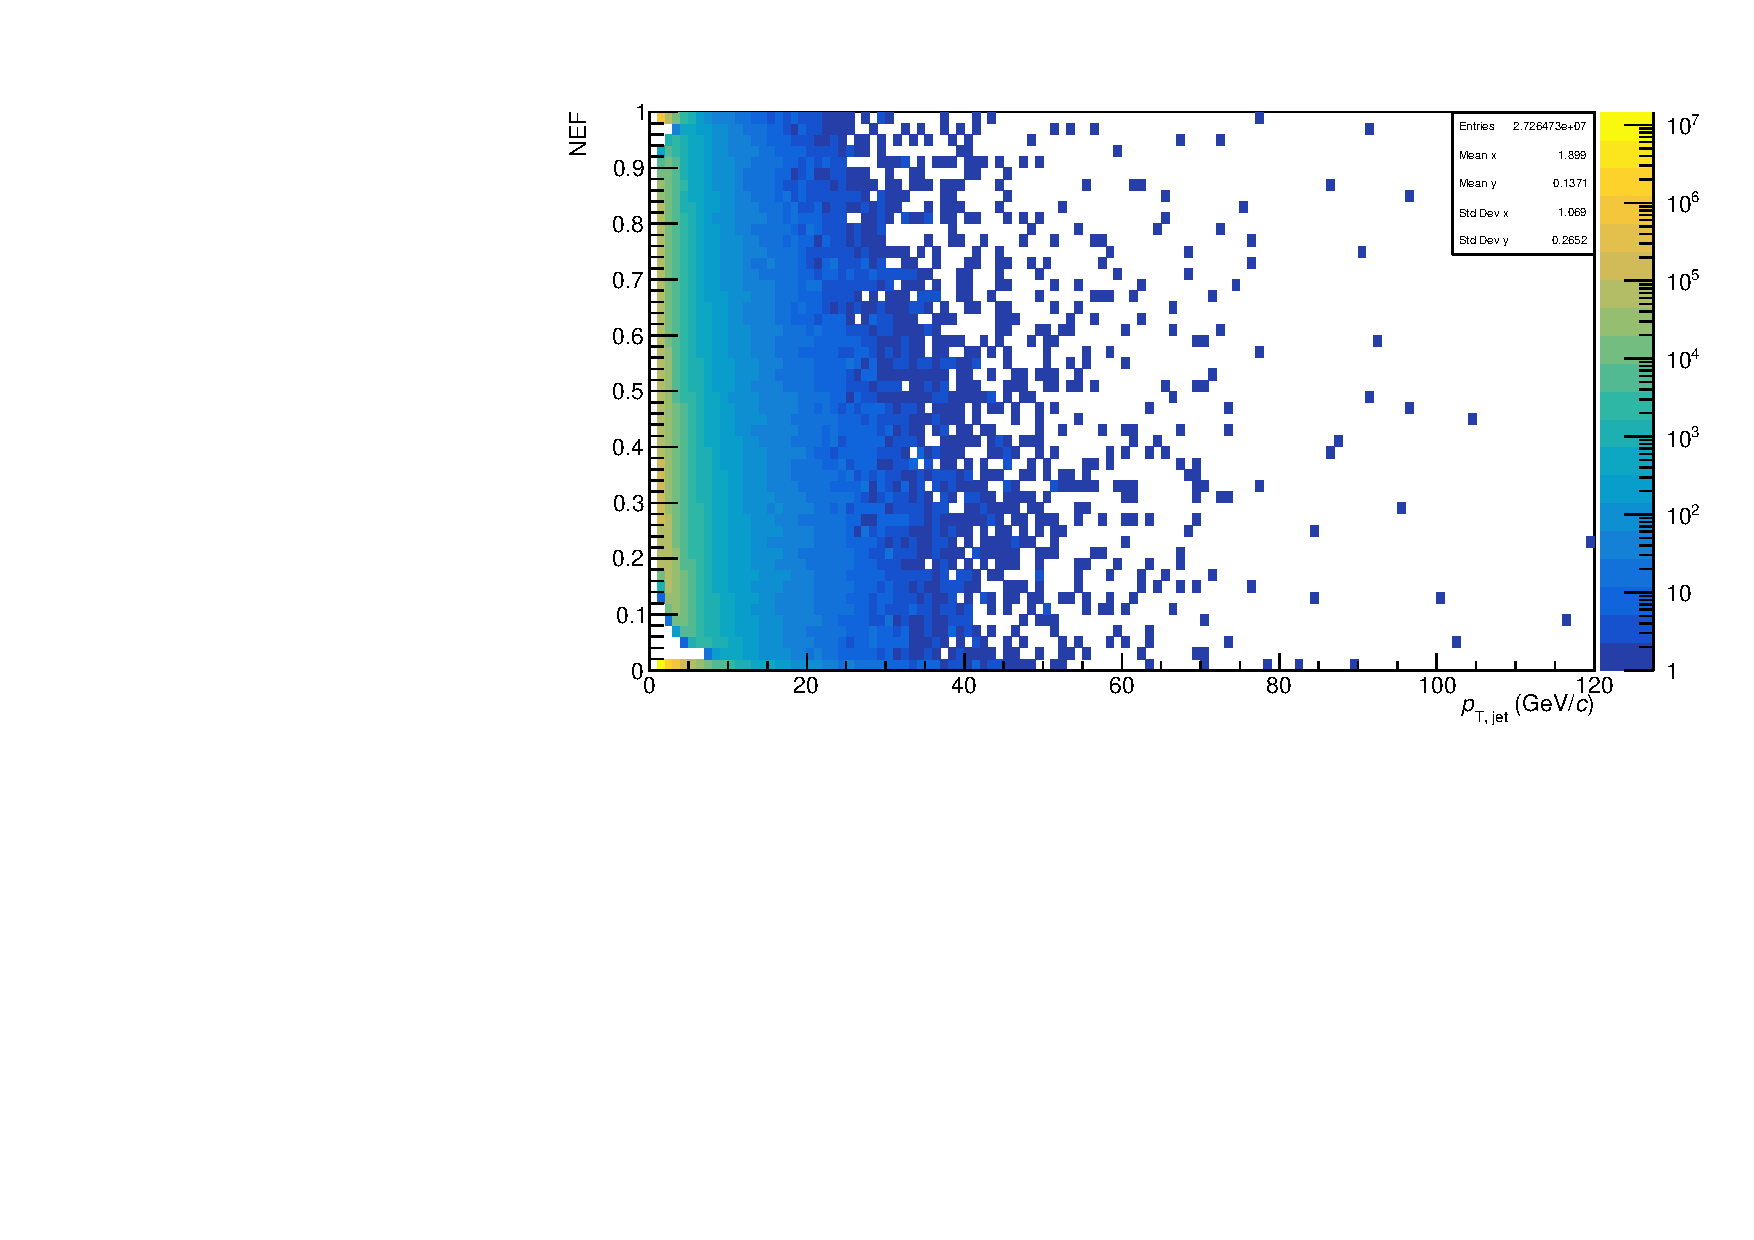
\includegraphics[width=13cm]{NEFR02}
\centering
\caption{R = 0.2 NEF per jet $P_{T}$.}
\label{fig:JetNEF}
\end{figure}




